%=========================================================================

\chapter{Introduction}

When does a machine understand an image? One definition could be the following sentence: \emph{A machine understand an image, when it can describe important content of the image.} This description should include present objects, their attributes and relation to each other. Determining the important content of the image can be quite difficult, even for humans, which have been trained for this task since they were born. However, deep learning techniques are proving to be quite successful in this kind of tasks. Similarly to people, these models require large amounts of training data, but, being properly trained, they can evaluate correctly even yet unseen situations.

Neural networks, sometimes mentioned under the name of deep learning, are a branch of machine learning based on composing multiple non-linear functions to solve the task. As it is fundamentally different from the standard computer algorithms, it perform well on problems, which are unsuitable for traditional solutions. For example, neural networks have excellent performance in recognizing speech and images, writing stories and composing music. This work focuses on generating image descriptions in regular English sentences, which is also a task suitable for deep learning.

First, chapter \ref{chp:nn} introduces neural networks and several key concepts, which are used later in this work. In chapter \ref{chp:captions} current state-of-the-art in the field of image captioning and summary of the key works will be presented. Equipped by knowledge from previous chapters, I will propose an image captioning model in chapter \ref{chp:design}. Overview of the programming tools used for implementing neural nets is in chapter \ref{chp:implementation}, as well as description of implementation of my model. Chapter \ref{chp:experiments} discusses experiments performed with my model, their results, and evaluation of the proposed solution. The concluding chapter \ref{chp:conclusion} serves as summary of the thesis and the important findings.

\chapter{Neural networks} \label{chp:nn}

General idea of artificial neural networks emerged after World War II. Perceptron, a single artificial neuron, was created in 1958 by Frank Rosenblatt~\cite{rosenblatt58a}, but it became popular only after combination with the backpropagation algorithm~\cite{bryson1975applied,werbos1974beyond}. At that time neural nets have not reached massive popularity, not because they do not work, but because small computing power of machines back then, and also the lack of datasets. Recently (after 2000), neural nets became popular again under the name of \textquotedblleft deep learning\textquotedblright to emphasize the use of several layers stacked on top of each other to create deep architectures, which are far more practical than shallow ones. During this reinvention, neural nets have been successfully applied in multiple fields like computer vision~\cite{DBLP:journals/corr/HeZRS15}, speech recognition~\cite{DBLP:journals/corr/abs-1303-5778}, and natural language modeling~\cite{DBLP:conf/interspeech/MikolovKBCK10}.

Nowadays, various useful architectures, techniques and applications of neural nets are introduced almost every day. As it is not possible to through all of them, in this chapter I will describe only a handful, which are most significant and will be later used in the research. This chapter is divided into three sections, each focusing on different type of neural nets --~feed-forward, recurrent, and convolutional. However, do not see this division as strict and separating, tools introduced in one part can and will be used in different types of networks.

\section{Feed-forward neural nets}

Feed-forward networks are simplest architecture of neural nets, yet they can solve many real world tasks. Most commonly used in classification problems, feed-forward nets showed very promising results, which later proved to be true. Later, they have been replaced by convolutional nets, which are specific type of complex feed-forward neural net. However, simple architectures still have place for utilization.

In this part I will cover linear neuron, rectifiers and other nonlinear functions used, and dropout, as they are most important to the following work. Other tools like softmax layer, loss functions, and training algorithms will be skipped.

\subsubsection{Linear unit}
In this type of neuron, the output of the unit is simply the weighted sum of its inputs added to a bias term, described by equation
\begin{align}
y \hspace{7pt}&=\hspace{7pt} Wx + b. \label{eq:lin}
\end{align}
A combination of these neurons performs a linear transformation of the input vector. Ability to perform only linear and affine transformations is also its weakness, as some kind of nonlinear function needs to be added to produce more complicated functions. However it is useful at the beginning and end of the network, to emphasize important features of the input or output and change its dimensionality.

This type of unit is the most basic one. It was part of the Rosenblatt's perceptron~\cite{rosenblatt58a} as well as the boolean function, which later evolved into nonlinear functions, like Rectifier described further.

\subsubsection{Rectifier and ReLU}

Combination of linear layers in neural network can result only in another linear layer, which is useless for example on problems of nonlinear separation. To break free from limitations induced, we need to introduce some kind of nonlinearity directly into the network. Most commonly used method is to apply a nonlinear activation function to the output of a linear neuron. As to which function, there are many suitable options, rectifier nowadays being the most popular one.

In the context of neural networks, the rectifier is an activation function defined as
\begin{align}
f(x) \hspace{7pt}&=\hspace{7pt} max(0,x). \label{eq:rectifier}
\end{align}
Rectifier is usually used after a linear unit creating together Rectified Linear Unit (\gls{relu}), which showed improvements in restricted Boltzmann machines~\cite{DBLP:conf/icml/NairH10}, speech processing~\cite{zeiler2013rectified}, and it is also default option in convolutional networks. This unit has several advantages against other functions -- in randomly initialized networks, only about 50\% of units are activated. There are no problems with vanishing gradient in large inputs. Computation of the function is also more efficient than other functions. Issue with this function is non-differentiability at zero, however it is differentiable at any point arbitrarily close to 0 and can be replaced with softplus~\cite{dugas2001incorporating}, which is analytic function smoothly approximating rectifier. Currently, more variations of \gls{relu} were introduced -- Leaky \gls{relu}, parametric \gls{relu}, etc. and their performance can be even better~\cite{DBLP:journals/corr/XuWCL15} than vanilla \gls{relu}s.

\begin{figure}[!t]
	\centering
	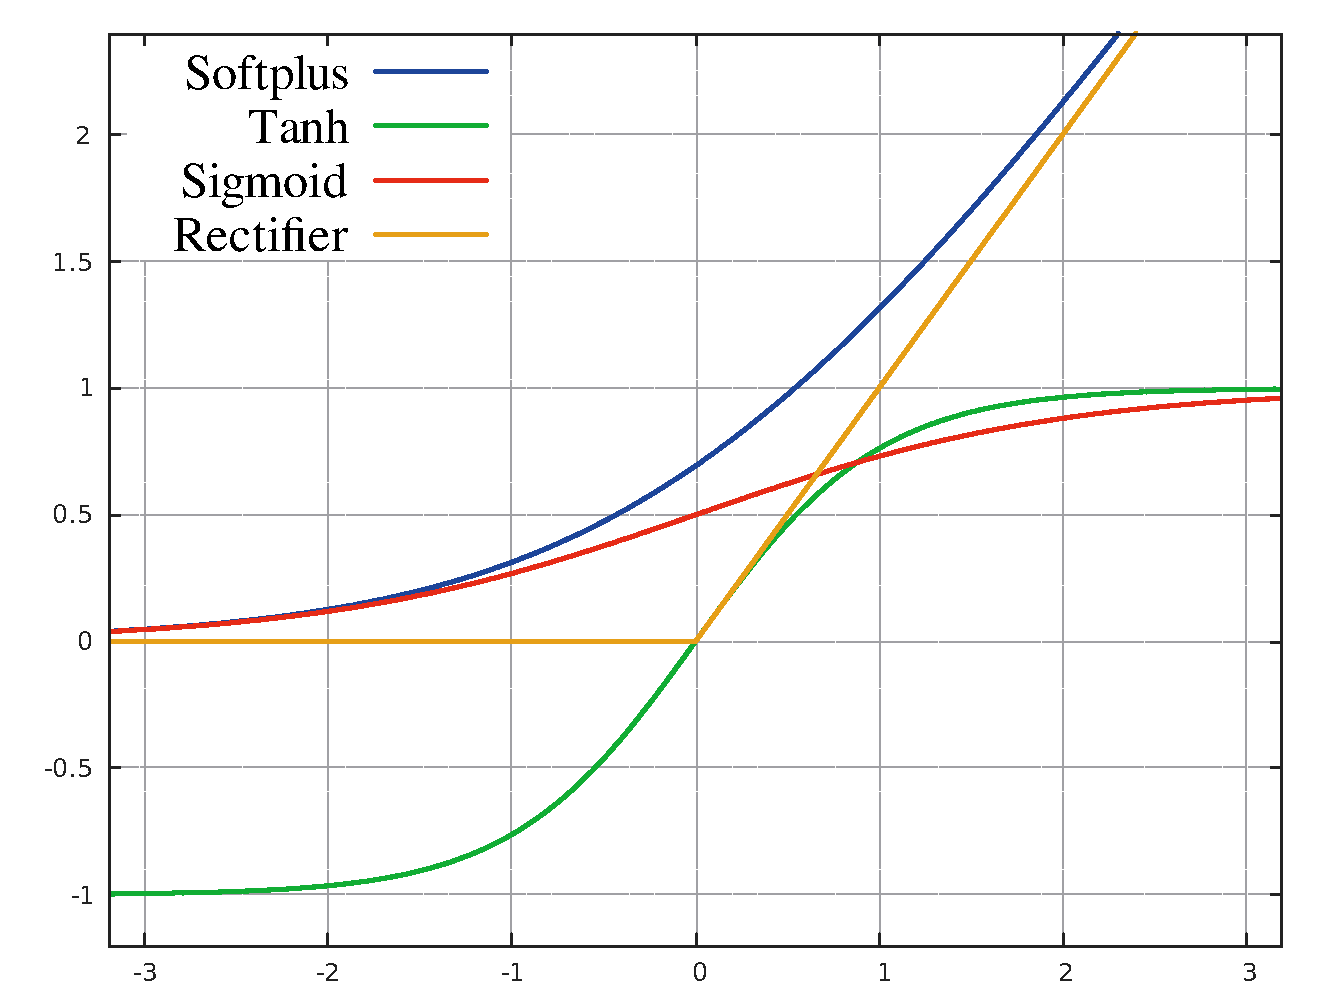
\includegraphics[width=0.6\textwidth]{fig/nonlinearities.pdf}
	\caption{Nonlinear functions used in neural nets.
		\label{fig:nonlinear}}
\end{figure}
Before \gls{relu}, popular functions were hyperbolic tangent and standard logistic function. However, these functions are costly to compute, even though they can be replaced with polynomials. Hyperbolic tangent was preferred as better version of logistic function~\cite{lecun2012efficient}. See how the discussed functions look at Figure \ref{fig:nonlinear}.

\subsubsection{Dropout}

Dropout~\cite{DBLP:journals/corr/abs-1207-0580, JMLR:v15:srivastava14a} can be considered as one of the biggest recent inventions in the field of neural networks. It is extremely simple and effective technique addressing the problem of overfitting. It can be seen as type of regularization, together with techniques like L1 and L2 regularization, and constraining maximum value of weights.

Dropout works with the idea of \textquotedblleft dropping out\textquotedblright\ some of the unit activations in a layer, that is setting them to zero, during training. This can be interpreted as sampling a neural network from the full neural network, and only updating the parameters of the sampled network for the given data. Visualisation is on Figure \ref{fig:dropout}, parts \emph{a} and \emph{b}. Dropout behaves differently during sampling phase -- all the units are present, but their outputs are multiplied by the same probability used before for dropping them out. See the part \emph{c} and \emph{d} of Figure \ref{fig:dropout}.

\begin{figure}[!t]
	\centering
	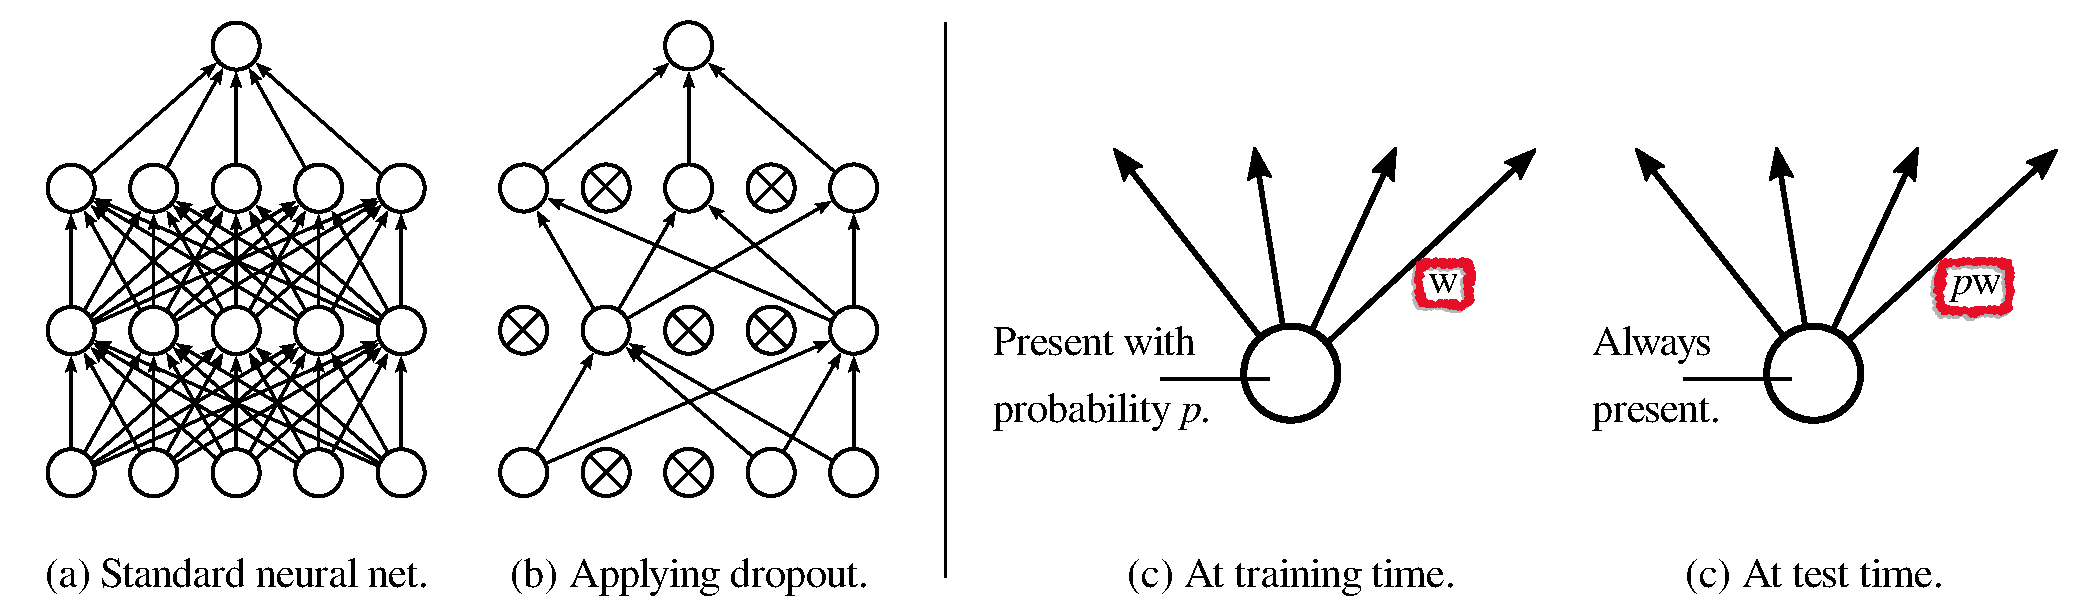
\includegraphics[width=0.9\textwidth]{fig/dropout.pdf}
	\caption{Applying dropout to a neural network.
		\label{fig:dropout}}
\end{figure}

This technique should prevent complex co-adaptations, in which unit is only helpful in the context of several other specific units. Each neuron instead learns to detect a feature generally useful for computing the answer.

\section{Recurrent neural nets}

Feedforward neural nets are extremely powerful models, but they can be only applied to problems with inputs and outputs of fixed dimensionality. This is a serious drawback, as many of the real-world problems are defined as sequences with lengths that are unknown to us beforehand. Recurrent neural networks were introduced soon after feed-forward nets and they proved to be very useful in this kind of a task. There is vast amount of recurrent neural network types, many not suitable for sequential tasks, like Hopfield networks~\cite{hopfield1982neural}, which are very successful in what they do, but nevertheless not useful for us now.

Apart from classification, which can be more precise when using sequences, one of the most important tasks is next value prediction. This core task can be then extended very simply to predict arbitrary number of future values. Prediction problems are all around us, from the weather forecast and stock market prediction to the autocomplete in smartphones or web browsers. The image captioning problem, which is the main topic in this work, includes the prediction (or generation) task too, as the caption is generated one character at a time starting from the \textquotedblleft base caption\textquotedblright. Detailed description is in the following chapters.

\begin{figure}[!t]
	\centering
	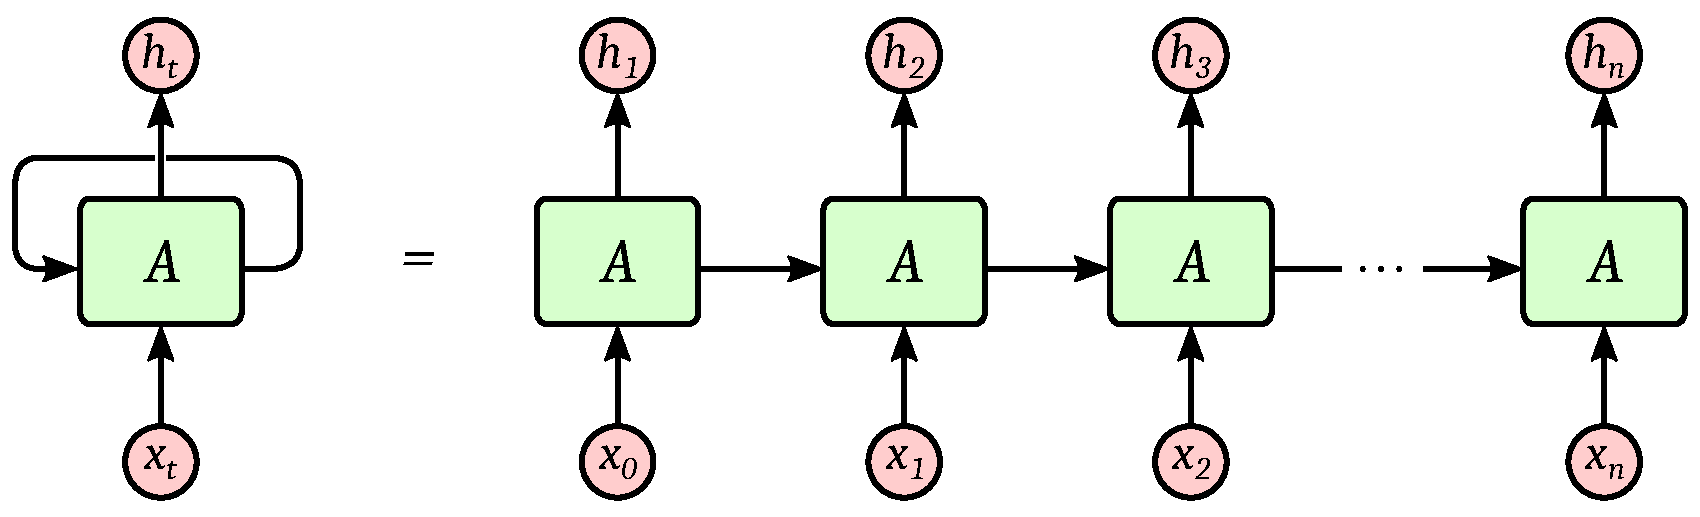
\includegraphics[width=0.9\textwidth]{fig/rnn-unrolled.pdf}
	\caption{Unrolling of a recurrent neural net.
		\label{fig:rnn-unroll}}
\end{figure}

We can interpret recurrent neural network as very deep forward net with shared weights and same inputs and outputs as before. This process of reinterpreting the network is called \gls{rnn} unrolling and is visualised in Figure \ref{fig:rnn-unroll}. Layers of this very deep net spread forward in time, together with the input sequence. This is very innovative idea, which enabled training \gls{rnn} with backpropagation through time, as we are not bound by time during training.

Unrolling the networks on long sequences and creation of very deep neural nets caused manifestation of the vanishing gradient problem, which is one of the most important issues in \gls{rnn}s. The problem occurs during training with gradient-based learning methods like backpropagation. The chain rule in backpropagation multiplies gradients  to compute updates of weights and the traditional activation functions like hyperbolic tangent have gradient in the range of $ (-1, 1) $, are the reasons why, the weights updates decrease exponentially while approaching front layers of the network. The vanishing gradient problem was formally identified by Hochreiter in 1991~\cite{hochreiter1991untersuchungen}, who, after further research, also proposed one of the solutions to this problem in the form of Long Short-Term Memory.

Long Short-Term Memory unit and other architectures commonly used in \gls{rnn}s are discussed in following section \ref{subsec:recUnits}. Second half (\ref{subsec:languageModels}) of this part explains how to process text and model languages for applications with \gls{rnn}s.

\subsection{Recurrent architectures}\label{subsec:recUnits}

\gls{rnn}s have many different architectures, however, most of them are derived from the basic fully recurrent network. This network do not have units separated into layers, as each of them has a directed connection to every other unit. Rest of the architectures are special cases of this one, as they group neurons into layers and implement only a subset of the connections. Examples of these architectures can be Hopfield~\cite{hopfield1982neural} and Elman~\cite{elman1990finding} networks, and Restricted Boltzmann Machines~\cite{Smolensky:1986:IPD:104279.104290}. Different architectures are trying to connect \gls{rnn} with an external memory resource, which can be a tape in case of Neural Turing Machines~\cite{DBLP:journals/corr/GravesWD14}, a stack in Neural network Pushdown Automata~\cite{Sun:1997:NNP:647638.733213}, etc. During training \gls{rnn} unrolling can be applied to these architectures, although training can be quite difficult, as explained earlier.

From here on in I will focus on an architecture called Long Short-Term Memory and architectures derived from it, as they are very powerful and dominating the current field.These units are carefully designed with the vanishing gradient problem in mind and perform better than most of the other architectures.

\subsubsection{Long Short-Term Memory}\label{subsubsec:lstm}

Long Short-Term Memory (\gls{lstm}) is a special type of recurrent network, able to learn long-term dependencies. This architecture was introduced by Hochreiter and Schmidhuber~\cite{Hochreiter:1997:LSM:1246443.1246450} after prior research of vanishing gradient problem, and later refined and popularized by other researchers~\cite{DBLP:conf/ijcnn/GersS00,DBLP:journals/neco/GersSC00}.

\gls{lstm} was designed to remember a value for an arbitrary length of time. It contains gates that determine, when the input is significant enough to remember, when it should keep or forget the value, and when it should copy the value to the output. To understand the flow of data, see the diagram of \gls{lstm} on Figure \ref{fig:lstm}. All the gates can be described by the following equations:
\begin{figure}[!t]
	\centering
	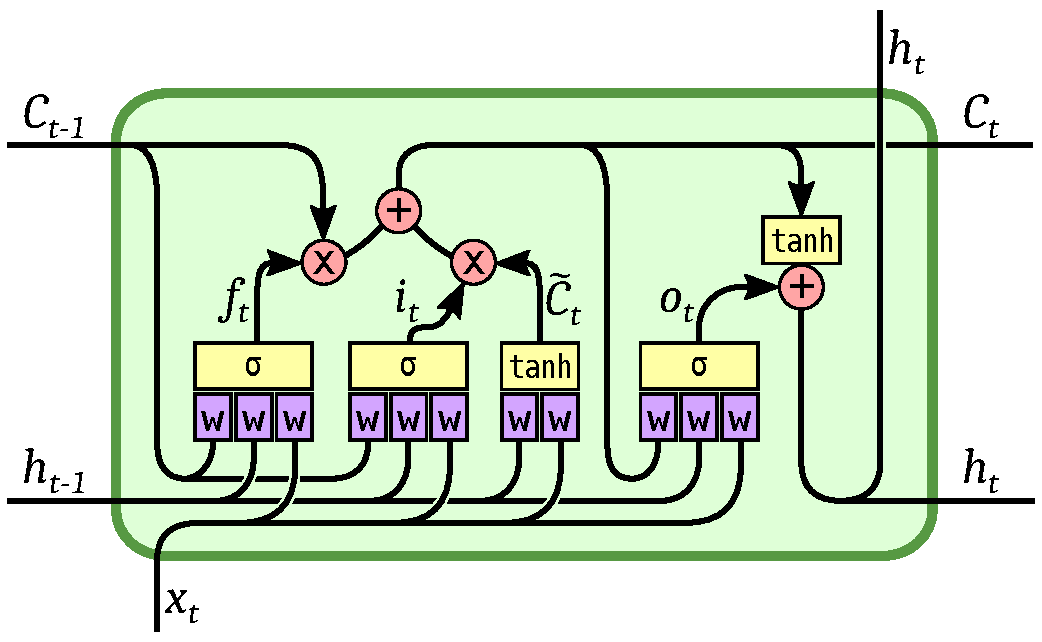
\includegraphics[width=0.7\textwidth]{./fig/lstm-peepholes.pdf}
	\caption{Variation of a \gls{lstm}.
		\label{fig:lstm}}
\end{figure}
\belowdisplayskip=16pt
\begin{align}
	i_t \hspace{7pt}&=\hspace{7pt} \sigma(W_{xi}x_t + W_{hi}h_{t-1} + W_{ci}C_{t-1} + b_i) \label{eq:lstm1}\\
	f_t \hspace{7pt}&=\hspace{7pt} \sigma(W_{xf}x_t + W_{hf}h_{t-1} + W_{cf}C_{t-1} + b_f) \label{eq:lstm2}\\
	\widetilde{C}_t\hspace{7pt}&=\hspace{7pt} \tanh(W_{xc}x_t + W_{hc}h_{t-1} + b_c) \label{eq:lstm3}\\
	C_t \hspace{7pt}&=\hspace{7pt} f_t\odot C_{t-1} + i_t\odot \widetilde{C}_t \label{eq:lstm4}\\
	o_t \hspace{7pt}&=\hspace{7pt} \sigma(W_{xo}x_t + W_{ho}h_{t-1} + W_{co}C_t + b_o) \label{eq:lstm5}\\
	h_t \hspace{7pt}&=\hspace{7pt} o_t\odot \tanh(C_t) \label{eq:lstm6}\\[16pt]
	\sigma(x) \hspace{7pt}&=\hspace{7pt} \frac{1}{1+e^{-x}} \label{eq:lstm7}
\end{align}
In each time slice \gls{lstm} is using current input $ x_t $, last cell state $ C_{t-1} $ and unit output $ h_{t-1} $ to compute next cell state $ C_t $ and output $ h_t $. Variables $ i_t $, $ f_t $, $ o_t $ denote values of in following order input, forget and output gates, which are used to control the information flow. LSTM based on these equations is using total of 11 weight matrices, 4 bias vectors, and a standard logistic function $ \sigma $ defined in Equation \eqref{eq:lstm7}. The operation $ \odot $ denotes element-wise vector product.

Equations \eqref{eq:lstm1} to \eqref{eq:lstm7} are not the only way to create an LSTM unit, they are a variation, which was used for implementing the proposed model. As \gls{lstm} is very popular, many different forms were created. For example, original \gls{lstm} from 1997~\cite{Hochreiter:1997:LSM:1246443.1246450} did not included the \textquotedblleft peephole connections\textquotedblright\ $ W_{ci}C_{t-1} $, $ W_{cf}C_{t-1} $, and $ W_{co}C_t $. These were added later in work of Gers and Schmidhuber~\cite{DBLP:conf/ijcnn/GersS00}. Another change is to couple input gate $ i_t $ and forget gate $ f_t $. Instead of separately deciding what to forget and when to input new information, unit only forgets the value when something new is placed in its place. More units based on \gls{lstm} and their comparison is in work of Greff, et al.~\cite{DBLP:journals/corr/GreffSKSS15}.

Training of the LSTM based network can be performed effectively by standard methods like stochastic gradient descend in the form of backpropagation through time. Major problem with vanishing gradients during training described earlier is not an issue as backpropagated error is fed back to each of the gates.

\subsubsection{Gated Recurrent Unit}\label{subsubsec:gru}

Gated Recurrent Unit (\gls{gru})~\cite{DBLP:journals/corr/ChoMGBSB14} is slightly more dramatic variation on the \gls{lstm} theme. It combines hidden state of the unit $ h_t $ with the saved value $ C_t $, merges input and forget gates into one update gate $ z_t $ and some smaller changes. Compare \gls{gru} diagram on Figure \ref{fig:gru} with the previous \gls{lstm} figure. \gls{gru} is based on following set of equations:
\begin{figure}[!t]
	\centering
	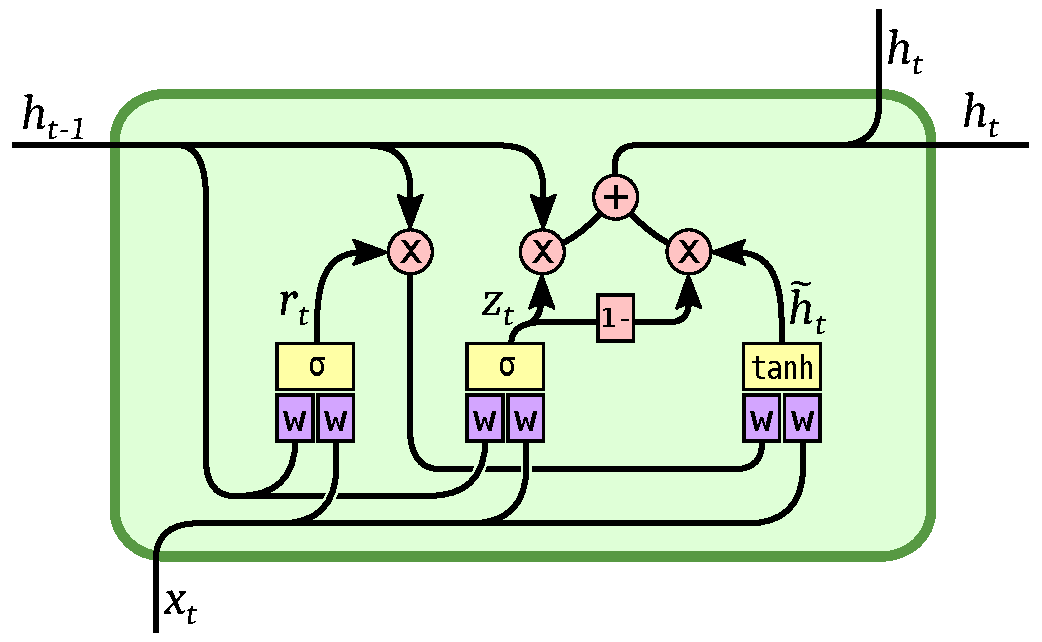
\includegraphics[width=0.7\textwidth]{./fig/gru.pdf}
	\caption{Variation of a GRU.
		\label{fig:gru}}
\end{figure}
\begin{align}
r_t \hspace{7pt}&=\hspace{7pt} \sigma(W_{xr}x_t + W_{hr}h_{t-1} + b_r) \label{eq:gru1}\\
z_t \hspace{7pt}&=\hspace{7pt} \sigma(W_{xz}x_t + W_{hz}h_{t-1} + b_z) \label{eq:gru2}\\
\widetilde{h}_t \hspace{7pt}&=\hspace{7pt} \tanh(W_{xh}x_t + W_{hh}(h_{t-1}\odot r_t) + b_h) \label{eq:gru3}\\
h_t \hspace{7pt}&=\hspace{7pt} (1-z_t)\odot \widetilde{h}_t + z_t\odot h_{t-1} \label{eq:gru4}
\end{align}
On top of the Equations \eqref{eq:gru1} to \eqref{eq:gru4}, \gls{gru} is using the standard logistic function $ \sigma $ defined in Equation \eqref{eq:lstm7}. The operation $ \odot $ again denotes the element-wise vector product. As the unit is using only 4 weight matrices, 3 biases and 1 state variable, researchers studied whether it can achieve the performance on same level as previous \gls{lstm}.

In Chung's study~\cite{DBLP:journals/corr/ChungGCB14}, different types of recurrent units were compared on the polyphonic music datasets. \gls{lstm} and \gls{gru} were performing significantly better than all of the other architectures, with \gls{gru} slightly in the lead. According to Greff, et al.~\cite{DBLP:journals/corr/GreffSKSS15} on the other hand, \gls{gru} is an average variation, slightly better than vanilla \gls{lstm}, with much simpler architecture.

Jozefowicz's study~\cite{DBLP:conf/icml/JozefowiczZS15} tried to determine whether the \gls{lstm} architecture is optimal and if such architecture exists. On variety of tasks and the data \gls{gru} outperformed \gls{lstm} on all tasks with the exception of language modeling. On top of that, they identified architectures that outperforms both \gls{lstm} and \gls{gru}. These architectures were found by evolutionary algorithm working on candidate architectures  represented by the computational graph. In this work I will explore different type of language modeling than the one used in Jozefowicz's paper~\cite{DBLP:conf/icml/JozefowiczZS15} and I will not focus on these new types of units. Interestingly they also confirmed that LSTM nearly matched the GRU's performance, when its forget gate bias was initialized to a large value such as 1 or 2, and not to naive initialization around 0. This idea was already presented by Gers \cite{DBLP:journals/neco/GersSC00} and can be interpreted in a way that \gls{lstm} will not explicitly forget anything until it has learned to forget.

Generally, researchers agree that most of the \gls{lstm} variations, including \gls{gru}, are roughly on the same performance level. As the changes introduced in \gls{gru} are simplifying the standard \gls{lstm} model even though keeping the performance level, \gls{gru} has been growing increasingly popular.

\subsection{Modeling languages}\label{subsec:languageModels}

With the addition of \gls{lstm}, recurrent neural nets quickly showed great potential in many different types of sequence processing like speech recognition, signal prediction and modeling languages. These result were further improved when researchers started stacking \gls{lstm}s on top of each other. Language modeling has several ways to process input text and feed it to the network. In this chapter, I will describe word and character level models, which are most commonly used.

%http://colah.github.io/posts/2014-07-NLP-RNNs-Representations/
Word level representation of the text is used by most of the state-of-the-art models, have been enhanced by many features and proved very effective for English. In this method, each word is encoded to a vector of a constant length. The neural network then works only with these encodings and does not have direct access to the word and its form. The advantage of this approach is no need to teach the model exact spelling of the words, which also means the model is not going to be confused by homographs\footnote{A \emph{homograph} is a word that shares the same written form as another word but has a different meaning.}. The benefit also is that encoded sequences are much shorter than sequences based on dividing text by character. On the other hand, the disadvantage of this approach is that modeling non-word text, like punctuation and long numbers, can be complicated.

All that is left, is to decide specific encoding for model to use.  Simple way that comes to mind is one-hot\footnote{One-hot encoded vector has exactly one high ('1') value and all the others low ('0').} or one-from-k encoding, which has its advantages, however, there are several issues with it in this application. The task vocabulary often exceeds 100 000 records, which means each input vector would be incredibly long. So long, issues with time complexity of computations would appear. Luckily set of techniques called \emph{word embedding} were developed. 

Word embedding~\cite{bengio2003neural} is a tool for mapping words or phrases from the vocabulary to suitable vectors of real numbers in low dimensional space (around 200 -- 500 dimensions) relative to the~vocabulary. For example,
\begin{align}
W(horse) \hspace{7pt}&=\hspace{7pt} (0.2,\ 0.4,\ 0.7,\ 0.1,\ \dots), \label{eq:embed1}\\
W(window) \hspace{7pt}&=\hspace{7pt} (0.0,\ 0.6,\ 0.1,\ 0.9,\ \dots). \label{eq:embed2}
\end{align}
Vectors are usually randomly initialized and then trained to capture structure of the input data to perform some task. An example can be skip-gram model~\cite{DBLP:journals/corr/abs-1301-3781}, which mapped 783 millions words to vectors of 300 real numbers, while creating reasonable relationships between them. Word embeddings show many interesting properties, like encoding analogies between words as differences between their vectors~\cite{export:189726}, but I am not going to cover them in more detail in this work.

Character level modeling has been considered as an alternative to word-level, but so far had worse performance. Regardless, it is still considered as an option, because of the much simpler representation of  the input and output. Consider roughly $ 45 $ characters in English text and over $ 100 000 $ words created from them. Same input can be modeled in character level by simple one hot encoding, instead of creating whole field of the word embeddings. These models are also more suited for Czech, Russian, and other fusional\footnote{Fusional language is a type of language distinguished by its tendency to overlay many morphemes to denote grammatical, syntactic, or semantic change.} languages, which heavily use prefixes and suffixes to create new words. 

Character level models usually have smaller vocabulary size and tend to take more time for training, as they need to learn spelling of the words and structure of a sentence, on top of the same features of word level. However, with the properly trained character level model, we can benefit from its greater generative abilities, on top of the very simple input and output of the model.

\section{Convolutional neural nets}

Feed-forward neural nets together with backpropagation algorithm have showed very useful for range of tasks and it has been even proven~\cite{cybenko:mcss,journals/nn/Hornik91} they can approximate any continuous function. However, they are not very good in recognizing objects presented visually. As every unit is connected to large amount of units in the previous layer (or all of them in fully-connected layers), the number of weights grows rapidly with the size of the problem and even more with the dimensionality. All these issues are becoming apparent even in image processing, which has only two dimensions. Convolutional neural nets (\gls{cnn}) were introduced as a way to reduce the number of parameters involved, while exploiting the spatial constraints of the input.

\gls{cnn} ideas took inspiration from neurobiology, more precisely the organisation of neurons in visual cortex of the cat. They were first used in the work of Homma~\cite{NIPS1987_20}, to process a temporal signal, and their design was later improved by LeCun et al.~\cite{lecun-98}. Different \gls{cnn} architecture was proposed by Graupe~\cite{graupe1988} for decomposing one-dimensional EMG signals\footnote{Electromyography (EMG) is an electrodiagnostic medicine technique for evaluating and recording the electrical activity produced by muscles.}. Convolutional nets can be also used in natural language processing~\cite{DBLP:journals/corr/Kim14f} and analysis of three-dimensional data like videos~\cite{10.1109/TPAMI.2012.59} or volumetric data (e.g. 3D medical scans), but that is not as common as image processing.

Basic architecture of \gls{cnn} can be described by the following process:

\begin{minipage}{0.9\textwidth}
\begin{enumerate}
	\setlength\itemsep{4mm}
	\item Convolve several small filters on the input.
	\item Subsample this space of filter activations.
	\item Repeat steps 1 and 2 until you are left with a sufficiently high level features.\label{itm:features}
	\item Use a standard feed-forward neural net to solve the task, using the features from step \ref{itm:features} as input.
\end{enumerate}
\end{minipage}
\vspace{9mm}

Thus the \gls{cnn} consist of alternating convolutional and subsampling layers, followed by fully-connected feed-forward network. Diagram of the simple \gls{cnn} architecture is on Figure \ref{fig:lenet}. I will now go through the individual network segments and describe them.

\begin{figure}[!t]
	\centering
	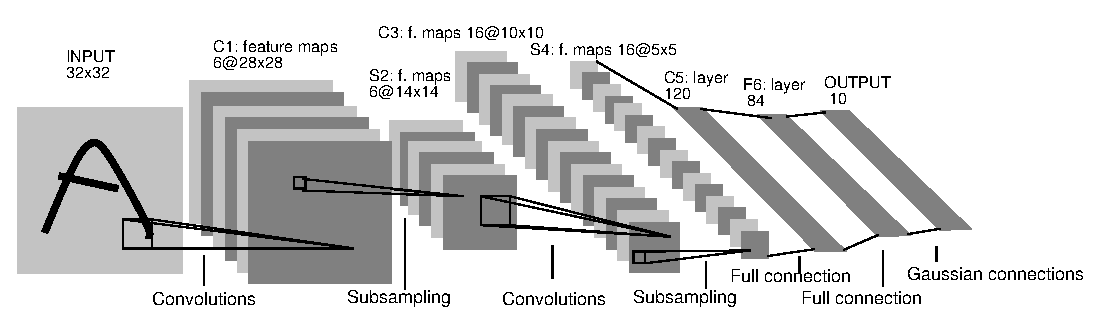
\includegraphics[width=\textwidth]{./fig/lenet.pdf}
	\caption{Architecture of famous \gls{cnn} \emph{LeNet-5}.~\cite{lecun-98}
		\label{fig:lenet}}
\end{figure}

Convolutional layer, which is most important and gave \gls{cnn}s their name, is essentially the same as mathematical convolution used elsewhere. Here it means to apply a 'filter' over an input at all possible offsets. This filter - in image processing and computer vision called kernel - has a layer of connection weights with the same dimensionality as the input, but with much smaller size. Despite the fact that there is many connections in one convolution, which are even overlapping, the weights are tied together and only handful of parameters per filter need to be updated during training. Usually, several filters, ranging from 5 to 100, are applied to the input simultaneously in one layer. The main reason why it is possible to use this architecture is the ability to stack convolutions on top of each other to create more high-level from low-level features, while keeping the proportions of input.

As the output of the network usually do not have same dimensions of the input, ability to directly control size of the features is needed. In \gls{cnn}s it is provided by subsampling, or in this version max pooling, layer. It is a simple operation that takes small non-overlapping grid of the input tensor and outputs the maximum value of each part. By putting this operation in between the convolutional layers, we can scale the current feature tensor and detect higher level features than without it.

Nowadays, most popular way to introduce nonlinearity to \gls{cnn} is inserting rectifiers after convolutions, as they have excellent performance, surpassing any other unit~\cite{jarrett-iccv-09, DBLP:conf/icml/NairH10}. In the second, fully-connected part, mix of linear units and \gls{relu}s is commonly used, with applying dropout to these layers. Connection between convolutional and fully-connected part is provided by a layer converting higher-dimensional output data from convolutions to a one-dimensional input vector.

\gls{cnn}s are useful in applications, where data has a spatial structure, which is useful to capture in the model. Among these data belongs image processing and speech recognition. One of the first and most famous examples of convolutional neural net is LeNet\footnote{Demos and examples of LeNet: \url{http://yann.lecun.com/exdb/lenet/}}~\cite{lecun-98}, which recognize handwritten digits from the MNIST database\footnote{MNIST database website: \url{http://yann.lecun.com/exdb/mnist/}}. Figure \ref{fig:lenet} shows the architecture of LeNet, version called \emph{LeNet-5}.

\chapter{Image Captioning}\label{chp:captions}

Scene understanding is one of the fundamental, but also most difficult tasks of computer vision and ability to automatically generate text captions of an image or video can have a great impact on lives of many. However, it is much more complicated than simple classification or object recognition tasks, because the model also need to understand relations between the recognized objects and encode that relationship correctly in the caption.

In this chapter, I have done an overview of state-of-the-art approaches to the image captioning task and more closely describe latest studies, which are the basis of this work (section \ref{sec:related}). Following section \ref{sec:datasets} cover popular datasets. Last section \ref{sec:evaluation} covers evaluation procedures, which are most commonly used for this task.

\section{Related Work}\label{sec:related}

Two main approaches to image captioning were popular, until neural networks dominated the field. The first one used caption templates, which were filled by detected objects and relations. Second was based on retrieval of similar captions from database and modifying them to fit the current image. Question of similarity ranking has been addressed by many papers, which are based on the idea of joint embedding vector space for both images and captions~\cite{DBLP:journals/corr/KarpathyF14}, as it transforms estimation of similarity to a simple proximity measurement. Both approaches included a generalization step to remove information relevant only to current image, for example names.

These approaches were quite successful in describing images, but they are heavily hand-designed. Also their text-generation power is fixated on the database/embeddings and is not able to describe previously unseen compositions of objects. Over time these approaches fell out of favor, as methods leveraging the power of neural networks emerged. However, some of their ideas proved to be useful in the new environment and we can encounter them in recent works~\cite{DBLP:journals/corr/FangGISDDGHMPZZ14}.

Many of the new methods, which use neural nets, are inspired by the success in training recurrent nets for machine translation. It is worth mentioning Sutskevers work ~\cite{DBLP:journals/corr/SutskeverVL14}, which studied general sequence to sequence mapping by converting an input sequence to the fixed length vector, which is then decoded to the output sequence. This encoder--decoder architecture is closely related to the autoencoders and work of Kalchbrenner and Blunsom~\cite{conf/emnlp/KalchbrennerB13}, who were first to map the entire input sequence to vector.

The introduced encoder--decoder architecture is important to the captioning task, because image description problem can be interpreted as a translation from an image to a sentence. In this case, encoder part of the model is usually a convolutional neural net, as they are excellent in the image classification~\cite{DBLP:journals/corr/SzegedyLJSRAEVR14}. Decoder part is the similar to the one in machine translation models -- an \gls{rnn} or a type of \gls{lstm}, as the output for both tasks is essentially the same.

Following the encoder--decoder idea, current image captioning research is shifting towards models, which are trained end-to-end with some type of stochastic gradient descent (\gls{sgd}) algorithm. The reasons for the shift can be simplicity and a lot less hand design than in other methods. Different type of the state-of-the-art models are based on proven pipeline of key-word detection, sentence generation, and ranking, which exploit the power of embedded neural networks, which specialize in single task. This approach is more closely described in section discussing article \emph{From Captions to Visual Concepts and Back}.

The current field is consolidating, thanks to \gls{coco} Captioning Challenge\footnote{\gls{coco} Captioning Challenge: \url{http://mscoco.org/dataset/\#captions-challenge2015}} and dataset created for it. Simple public access to the necessary data makes model creation easier and the best researchers can compete directly against each other by using \gls{coco} evaluation server. In the rest of this section, I describe several works, which were submitted to the challenge in 2015 and had the best performance. \gls{coco} dataset is described, together with other datasets, in following section \ref{sec:datasets}.

\subsubsection{Show and Tell: A Neural Image Caption Generator}

\emph{Show and Tell}~\cite{DBLP:journals/corr/VinyalsTBE14} is model created by Google researchers, which tied for the first place in \gls{coco} Captioning Challenge with the following model \emph{From Captions to Visual Concepts}. The main idea of this work is to use recent advancements in machine translation and apply them for image captioning. Model uses encoder--decoder architecture, with \gls{cnn} for the encoder part and \gls{rnn} for the decoder part, as described earlier. Model is trained to maximize the likelihood $ p(S|I) $ of producing a target sequence of words $ S = \{S_1,S_2,...\} $ given an input image $ I $.

Used convolutional neural net has been pre-trained for an image classification task and last hidden layer of this network has been used as an input to the \gls{rnn} decoder. The \gls{rnn} part of the network is made of \gls{lstm} units based on following equations:
\begin{align}
i_t \hspace{7pt}&=\hspace{7pt} \sigma(W_{xi}x_t + W_{hi}h_{t-1}) \label{eq:showlstm1}\\
f_t \hspace{7pt}&=\hspace{7pt} \sigma(W_{xf}x_t + W_{hf}h_{t-1}) \label{eq:showlstm2}\\
\widetilde{C}_t \hspace{7pt}&=\hspace{7pt} \tanh(W_{xc}x_t + W_{hc}h_{t-1}) \label{eq:showlstm3}\\
C_t \hspace{7pt}&=\hspace{7pt} f_t\odot C_{t-1} + i_t\odot \widetilde{C}_t \label{eq:showlstm4}\\
o_t \hspace{7pt}&=\hspace{7pt} \sigma(W_{xo}x_t + W_{ho}h_{t-1}) \label{eq:showlstm5}\\
h_t \hspace{7pt}&=\hspace{7pt} o_t\odot C_t \label{eq:showlstm6}
\end{align}
Notation is same as in the chapter \ref{chp:nn}, $ \sigma $ is the standard logistic function defined in Equation \eqref{eq:lstm7} and the operation $ \odot $ denotes the element-wise vector product. It is worth noticing the \gls{lstm} version used do not have \textquotedblleft peephole connections\textquotedblright. Several more changes were added~-- the second evaluation of hyperbolic tangent in Equation \eqref{eq:showlstm6} is missing, as well as biases in all equations.

\begin{figure}[!t]
	\centering
	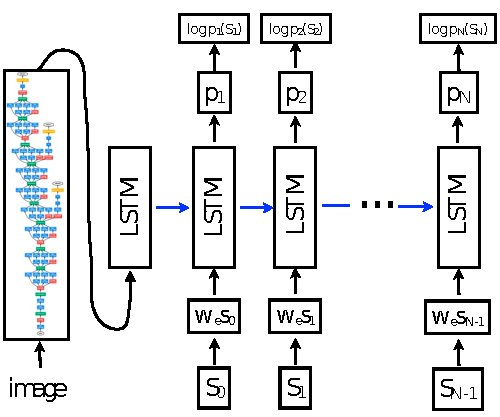
\includegraphics[width=0.6\textwidth]{./fig/show-tell_model.pdf}
	\caption{\emph{Show and Tell} image captioning model.~\cite{DBLP:journals/corr/VinyalsTBE14}
		\label{fig:showmodel}}
\end{figure}

The language model is working on the word-level, part of the \gls{rnn} is word embedding~\cite{DBLP:journals/corr/abs-1301-3781}, which is trained together with the model. \gls{cnn}, which is used to generate a configuration vector from the image, is connected to the \gls{rnn} at the beginning as the first input before the generated sequence. Overall structure of the model is visualized on Figure \ref{fig:showmodel} and can be represented by following equations:
\begin{alignat}{3}
x_{-1}  \hspace{7pt}&=\hspace{7pt} CNN(I)& \label{eq:showmodel1}\\
x_t     \hspace{7pt}&=\hspace{7pt} W_eS_t \hspace{20pt} & t\in\{0\ldots N-1\}  \label{eq:showmodel2}\\
p_{t+1} \hspace{7pt}&=\hspace{7pt} LSTM(x_t) \hspace{20pt} & t\in\{0\ldots N-1\}  \label{eq:showmodel3}
\end{alignat}
As the image and word encodings are used in the same way, model is effectively mapping both images and words into the same vector space. During the sequence input, special start word $ S_0 $ and stop word $ S_N $ designated to mark start and end of the sequence are used.

The CNN component of the model has been initialized to an ImageNet trained model, which helped quite a lot in terms of generalization. Word embeddings were left uninitialized (initialized randomly) as they did not observed significant gains while using large corpus. Dropout and ensebling used during training gave minor improvements. Model has been trained using \gls{sgd} with fixed learning rate and no momentum. For the embeddings vector and the LSTM memory 512 dimensions were used. During the inference, beam search has been used to improve the results.

\subsubsection{From Captions to Visual Concepts and Back}

This work~\cite{DBLP:journals/corr/FangGISDDGHMPZZ14} took quite a different approach than a previous one, however, both tied for the first place in the captioning competition. This model is not trained end-to-end with a single training algorithm rather it has three connected stages. Full pipeline of the model is on the Figure \ref{fig:fromCaptionsModel} and its description follows.

\begin{figure}[!t]
	\centering
	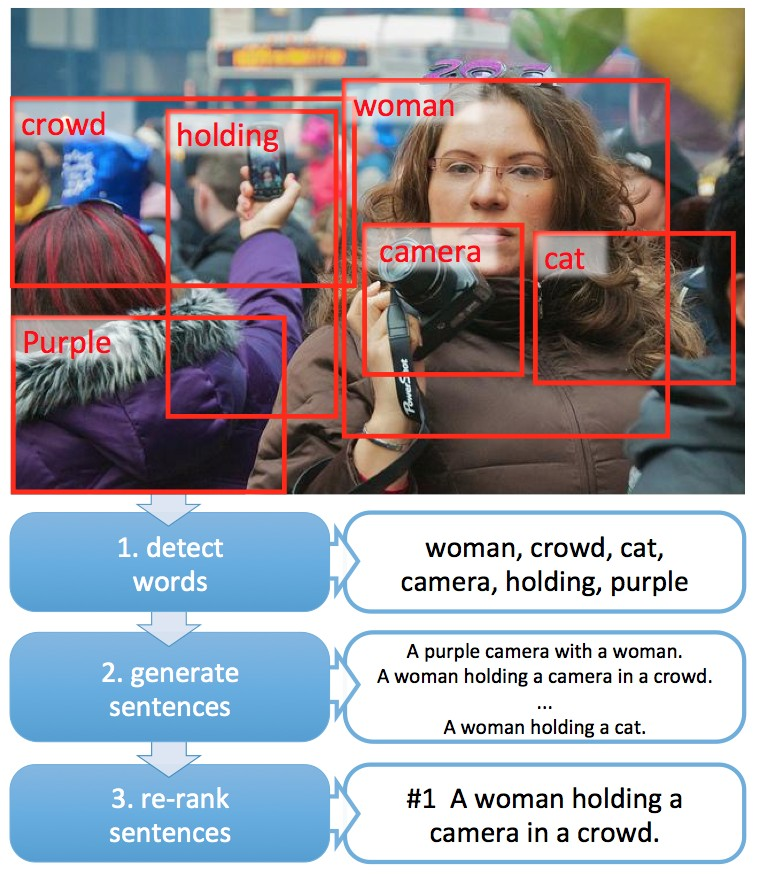
\includegraphics[width=0.5\textwidth]{./fig/from-captions-workflow.png}
	\caption{\emph{From Captions to Visual Concepts} caption generation pipeline.~\cite{DBLP:journals/corr/FangGISDDGHMPZZ14}
		\label{fig:fromCaptionsModel}}
\end{figure}

First, model learns to extract nouns, verbs, and adjectives by applying \gls{cnn} to regions of the image. These words come from the vocabulary constructed with 1000 most common words in the training captions. By running detector on the image regions, model is able to produce a bag of bounding boxes, which represent the location of the appropriate word in the image. Network used for the word detection is the 16-layered \gls{cnn}, commonly referred as \gls{vgg}, from a conference paper~\cite{DBLP:journals/corr/SimonyanZ14a}.

Second stage use the extracted words to guide a language model to generate sentences likely  to describe the image. The maximum entropy language model estimates the probability of a word $ w_i $ conditioned on the preceding words as well the words with high likelihood detections, yet to be mentioned. This encourages all the words to be used, while avoiding repetitions. A left-to-right beam search is used during generation. After extending each sentence with a set of likely words, the top $ N $  sentences are retained and the others pruned away. The process continues until a maximum sentence length $ L $ is reached.

In the third stage, candidate captions are re-ranked using Minimum Error Rate Training~\cite{och2003minimum} (\gls{mert}) and the best one is selected. \gls{mert} uses a linear combination of features computed over the sentence, for example log-likelihood of the sequence or its length. One of the features is Deep Multimodal Similarity Model (\gls{dmsm}) score, which measures similarity between images and text. The \gls{dmsm} has been proposed in this paper and the model trains two neural networks that map images and text fragments to a common vector representation. These vectors are used to compute the cosine similarity score, which is then sent to \gls{mert}.

As mentioned earlier, this model is the state-of-the-art on the \gls{coco} Captioning Challenge, as it tied for the first place with the \emph{Show and Tell} work. Their final and best performing model used \gls{vgg}, word detector score in maximum entropy language model, proposed \gls{dmsm} and use finetuned \gls{vgg} features. According to human judgment, generated captions are equal to or better than human-written captions 34\% of the time.

Direct comparison of the \emph{From Captions to Visual Concepts} approach with the \emph{Show and Tell}, which was presented earlier, is in the additional article~\cite{DBLP:journals/corr/DevlinCFGDHZM15} by the same authors. They examine the issues of both approaches and achieve state-of-the-art performance by combining key aspects of \gls{rnn} and maximum entropy methods.

\subsubsection{Show, Attend and Tell: Neural Image Caption Generation with Visual Attention}

\emph{Show, Attend and Tell}~\cite{DBLP:journals/corr/XuBKCCSZB15} is method, made by researchers from universities in Toronto and Montreal, which introduced an attention based model. Attention is one of the most interesting parts of the human visual system. Rather than compressing an entire image into a static representation, attention allows for salient features to dynamically come to the forefront as needed. Proposed model has encoder-decoder architecture with feedback connections for attention. Overall structure of the model is on Figure \ref{fig:attendmodel}. Encoder part use a \gls{cnn} to extract set of feature/annotation vectors (not just one). Each of the vectors correspond to a part of image. To obtain a correspondence between them, features from a lower convolutional layer are used.

\begin{figure}[!t]
	\centering
	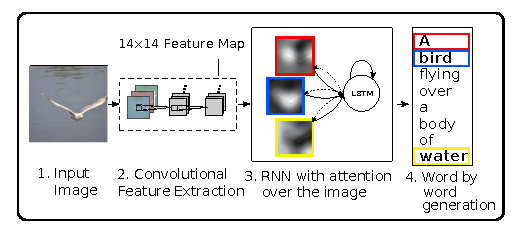
\includegraphics[width=0.7\textwidth]{./fig/show-attend-tell_model.pdf}
	\caption{\emph{Show, Attend and Tell} model architecture.~\cite{DBLP:journals/corr/XuBKCCSZB15}
		\label{fig:attendmodel}}
\end{figure}

Decoder part is a \gls{lstm} network working of the word level, which generates, apart from the word of the output, a context vector - a dynamic representation of the relevant part of the image at time $ t $. The paper explored two attention mechanisms computing the context vector from the annotation vectors. First is the stochastic \textquotedblleft hard\textquotedblright\ mechanism, which interprets the values in the context vector as the probability that corresponding location is the right place to focus, while producing the next word. Second is deterministic \textquotedblleft soft\textquotedblright\ mechanism introduced in~\cite{DBLP:journals/corr/BahdanauCB14}, which gives the relative importance of the location by blending values of all annotation vectors together. This method is fully trainable by the standard \gls{sgd} methods.

\begin{figure}[!t]
	\centering
	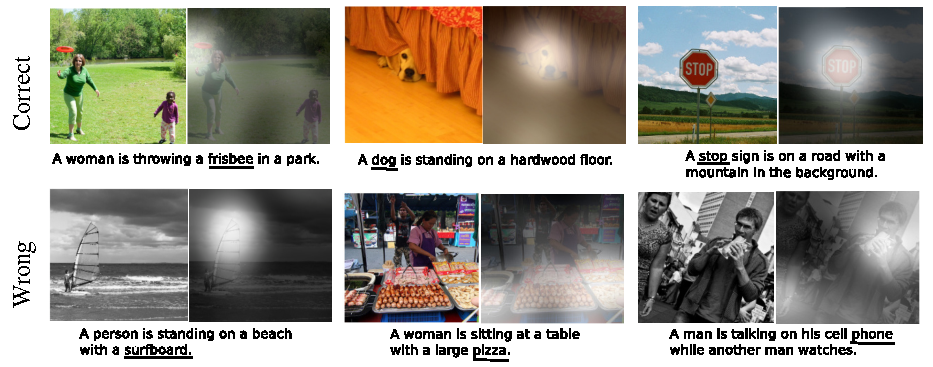
\includegraphics[width=0.95\textwidth]{./fig/show-attend-tell_example.pdf}
	\caption{Examples of \emph{Show, Attend and Tell} attention.~\cite{DBLP:journals/corr/XuBKCCSZB15}
		\label{fig:attendexample}}
\end{figure}

Article also shows how we can gain insight and interpret the results of the model by visualizing where and on what was the attention focused. Examples of the attention visualizations with both, correct and wrong generations, are on Figure \ref{fig:attendexample}. Visualizations show that the model can attend even a \textquotedblleft non-object\textquotedblright\ regions. This adds an extra layer of interpretability to the output. The model learns alignments that correspond very strongly with human intuition and, even, in the cases of mistakes, we can understand why the captions were generated.

Similarly to previous article, \emph{Show, Attend and Tell} used \gls{vgg}~\cite{DBLP:journals/corr/SimonyanZ14a}, a \gls{cnn} trained on the ImageNet, which was not finetuned. Model was trained with several algorithms and researchers found that for Flickr8k dataset, RMSProp worked best, while for Flickr30k and MSCOCO datasets, Adam~\cite{DBLP:journals/corr/KingmaB14} algorithm was used. Performance during training was also improved by creating minibatches of sentences with same length, which greatly improved convergence speed.

\subsubsection{Long-term Recurrent Convolutional Networks for Visual Recognition and Description}

The research group from Berkeley presented \emph{Long-term Recurrent Convolutional Networks} (\gls{lrcn})~\cite{DBLP:journals/corr/DonahueHGRVSD14}, which combines network  with convolutional and long-range temporal layers for several tasks. It is possible to apply \gls{lrcn} to recognize activity performed on the video (sequential input $ \mapsto $ fixed output), generate description  of the image (fixed input $ \mapsto $ sequential output) or describe video (sequential input $ \mapsto $ sequential output).

\begin{figure}[!t]
	\centering
	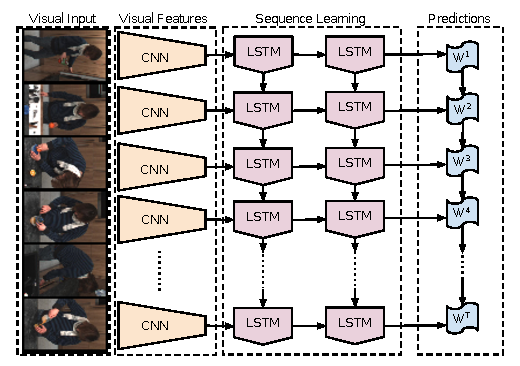
\includegraphics[width=0.65\textwidth]{./fig/long-term-rec-con_architecture.pdf}
	\caption{The \gls{lrcn} model architecture for video processing.~\cite{DBLP:journals/corr/DonahueHGRVSD14}
		\label{fig:lrcn}}
\end{figure}

Architecture of the proposed model, see Figure \ref{fig:lrcn}, is similar to the \emph{Show, Attend and Tell}, as image is processed by \gls{cnn} and sent to the input of the \gls{lstm} in each time step. Feedback attention connections are missing in this model. According to the task specification, method can use separate convolutional networks, different for each time step with specific input, or single \gls{cnn} throughout all the time steps.

\gls{lrcn} tied with \emph{Show, Attend and Tell} in \gls{coco} Captioning Challenge for the third place. However, this does not mean the models are equal in general performance, as each of them focuses on different research topic.

\section{Datasets}\label{sec:datasets}

Large amounts of data are necessary requirement in training deep neural nets like  \gls{cnn}s and \gls{rnn}s, as well as sufficient computing power. Access to the machines and hardware suitable for training has been made in recent years extremely easy, with the rise of virtualization services. Obtaining enough data is different issue and it is currently the biggest problem. Especially, creation of image captioning datasets is quite complicated. As there is no automatized way to generate data, all the image descriptions have to be human-generated. This is one of the reasons, only few specialized datasets are created.

There are two main options how to get images and captions. First way is, by using user-generated data from an online service, most commonly Flickr\footnote{Flickr is a popular image hosting website and an online community. (\url{https://www.flickr.com})}. However, these captions are not made specifically for the task and could be prone to error. Second option is to gather only images, again from Flickr or other online services, and create captions for direct use in the dataset manually. Amazon Mechanical Turk\footnote{Amazon Mechanical Turk is crowdsourced Internet marketplace for tasks that computers are currently unable to do. (\url{https://www.mturk.com})} is heavily used for this task.

Following Table \ref{tab:datasets} lists the most popular datasets. All these datasets were created directly for the image captioning task, with captions generated through Amazon Mechanical Turk. Flickr8k~\cite{dataset-flickr8k}, from 2013, was one of the first datasets created for this purpose. It has been later expanded into Flickr30k~\cite{dataset-flickr30k}. The biggest dataset is Microsoft Common Objects in Context (\gls{coco})~\cite{DBLP:journals/corr/ChenFLVGDZ15}, created for the \gls{coco} captioning challenge. CIDEr~\cite{Vedantam_2015_CVPR} datasets PASCAL-50S, ABSTRACT-50S are youngest mentioned, designed specifically for evaluation with the CIDEr metric discussed in section \ref{sec:evaluation}.

\def\arraystretch{1.2}%  1 is the default, change whatever you need
%\setlength\extrarowheight{20pt}%add points to the row height

\begin{center}
	\begin{longtable}{|l|m{2cm}|m{2cm}|m{4.7cm}|}
		\caption{Image captioning datasets.} \label{tab:datasets} \\

	   	\hline
	   	\multicolumn{1}{|l|}{\textbf{Name}} &
	   	\textbf{Images} &
	   	\textbf{Captions per image} &
	   	\textbf{Note} \\
	   	\hline \hline
		\endhead

	   	MS COCO\footnote{MS COCO project: \url{http://mscoco.org/dataset/}} &
		   	\multicolumn{1}{r|}{123 287} &
		   	\multicolumn{1}{c|}{5} &
		   	Images are divided - 82 783 for training and 40 504 for testing purposes. \\ \hline
	   	Flickr30k\footnote{Flickr30k project: \url{http://shannon.cs.illinois.edu/DenotationGraph/}} &
		   	\multicolumn{1}{r|}{31 783} &
		   	\multicolumn{1}{c|}{5-6} &
		   	An extension of Flickr8k dataset. \\ \hline
	   	Flickr8k\footnote{Flickr8k project: \url{http://nlp.cs.illinois.edu/HockenmaierGroup/8k-pictures.html}} &
		   	\multicolumn{1}{r|}{8 092} &
		   	\multicolumn{1}{c|}{5} &
		   	Focused on people or animals (mainly dogs) performing some specific action. \\ \hline
	   	PASCAL-50S\footnote{\label{ft:cider}PASCAL-50S and ABSTRACT-50S: \url{http://ramakrishnavedantam928.github.io/cider/}} &
		   	\multicolumn{1}{r|}{1 000} &
		   	\multicolumn{1}{c|}{50} &
		   	Built upon images from the UIUC Pascal Sentence Dataset. \\ \hline
	   	ABSTRACT-50S\footnote{See footnote \ref{ft:cider}.} &
		   	\multicolumn{1}{r|}{500} &
		   	\multicolumn{1}{c|}{50} &
		   	Built upon images from the Abstract Scenes Dataset. No photos.\\ \hline
	\end{longtable}
\end{center}

\section{Evaluation}\label{sec:evaluation}

Recent progress in fields like machine translation, which are very similar to image captioning, caused spike of interest in evaluating regular text output accuracy. Although, sometimes it is not clear, if a description of an image is the best option available, some degree of assessment is possible. The best results can be obtained by asking live raters to score the usefulness of each description. Subjective scores can vary, but their average over many raters are usually quite accurate. However, this method consumes tremendous amount of time and external raters are necessary in most cases. Like with data generation, tools like Amazon Mechanical Turk are used to great extent, but need for automated tools is evident.

\subsection{Automated metrics}

Assuming that one has access to human-generated captions, which is ground truth in our case, completely automated metrics are available. Even though all of them compute how alike are model descriptions to human-generated, different ratings are used by different metrics and even differences between used settings and implementations of one metric can invalidate the results. This raises the question, how can we compare results of different works, despite them using the \textquotedblleft same\textquotedblright\ evaluation method. Microsoft group of researchers, team responsible for \gls{coco}, addresses this issue in~\cite{DBLP:journals/corr/ChenFLVGDZ15}. They created an evaluation server\footnote{\gls{coco} evaluation server: \url{http://mscoco.org/dataset/\#captions-upload}.}, which has many automated metrics, with several configurations, including all mentioned here. This server should serve as a reference point for comparison of image captioning models.

Among the most popular metrics belong \gls{bleu}, \gls{meteor}, and \gls{cider}. The rest of this section is describing and discussing their properties. \gls{bleu} (Bilingual Evaluation Understudy)~\cite{Papineni:2002:BMA:1073083.1073135} has been the most commonly used metric, which was created in 2002 to evaluate quality of machine translated text. Scores are computed on individual segments, usually sentences. \gls{bleu} has high correlation with human judgments and is very popular, even for captioning tasks. However, it is becoming outdated, as according to this metric, automatic methods are now outperforming humans, which is senseless. Four different variations of \gls{bleu} are used in \gls{coco} evaluation server.

\gls{meteor} (Metric for Evaluation of Translation with Explicit Ordering)~\cite{Lavie:2007:MAM:1626355.1626389} is another metric for the evaluation of machine translation, slightly younger than \gls{bleu}, from 2007. Scoring generated translations is performed by aligning them to one or more reference translations. Metric was designed to fix some problems of the \gls{bleu}. It can also look for synonyms and perform stemming on input words.

Metric designed directly to caption evaluation -- \gls{cider} (Consensus-based Image Description Evaluation)~\cite{Vedantam_2015_CVPR} was introduced in 2015. This is still a very new metric, but with growing popularity as it correlate well with human judgment. Main idea of this metric is improving quality of the metric with growing number of captions for the single image. This can be observed on datasets introduced with it (see section \ref{sec:datasets}).

\chapter{Model design}\label{chp:design}

In the previous chapters, the basics of creating neural networks have been laid down, with special focus on \gls{rnn} units like \gls{lstm} and \gls{gru}, and \gls{cnn}s. Chapter \ref{chp:nn} also included description of trends in language modeling with \gls{rnn}s - word and character level models. Following chapter \ref{chp:captions} described the current approaches to image captioning and how are state-of-the-art models designed. Chapter also introduced most popular image captioning datasets and evaluation metrics in a short list.

Equipped with the knowledge of previous chapters. In is chapter I will propose the architecture of an image captioning model and describe in detail each part and their connections (section \ref{sec:overallArch}). Second part of this chapter (section \ref{sec:training}) is about training procedure of the proposed model - which algorithms and datasets are used, and other details.

\section{Overall architecture} \label{sec:overallArch}

As a result of the previous research, I designed an image captioning model with the encoder--decoder architecture, slightly based on the \emph{Show and Tell}~\cite{DBLP:journals/corr/VinyalsTBE14}  and \emph{Show, Tell and Attend}~\cite{DBLP:journals/corr/XuBKCCSZB15} models. In this section I describe the \gls{cnn} encoder part of the model, then, in separate sections \ref{subsec:designLangMod} and \ref{subsec:initialization}, \gls{rnn} modeling language and how to feed the image encoding to the \gls{rnn}. Throughout the section, all the descriptions refer to the diagram on Figure \ref{fig:proposedModel}, as each of them discuss different parts of the image.

\begin{figure}[!t]
	\centering
	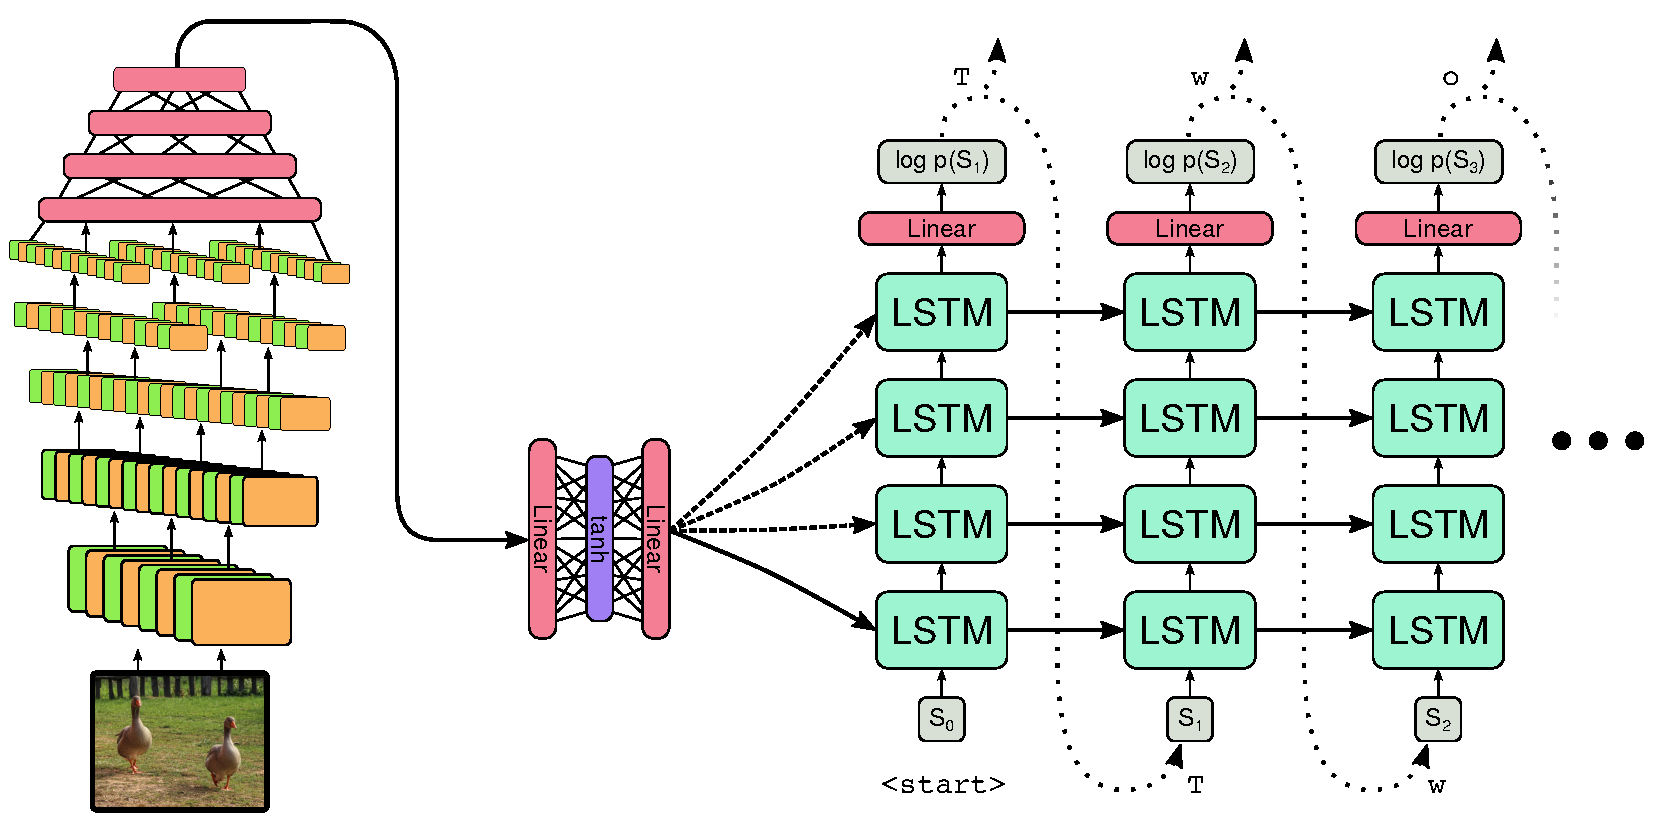
\includegraphics[width=\textwidth]{./fig/proposed-model.pdf}
	\caption{Architecture of the proposed model.
		\label{fig:proposedModel}}
\end{figure}

The \gls{cnn} used in this model is \gls{vgg}~\cite{DBLP:journals/corr/SimonyanZ14a} - a 16-layer network trained on ImageNet. The same one as the one in \emph{From Captions to Visual Concepts} and \emph{Show, Attend and Tell} papers. Input of the \gls{cnn} is a fixed-size $ 224 \times 224 $ RGB image, which passes through a stack of convolutional layers with very small receptive fields: $ 3 \times 3 $, and rectifiers. Throughout the network, some of the convolutional layers are followed by max-pooling. 

Original network produces a probability distribution over 1000 ImageNet classes. For my purposes, I removed the last \emph{softmax} layer, as well as last fully-connected layer \emph{fc8}, which is the approach used by \emph{From Captions to Visual Concepts}. Thus, output of the \gls{cnn} has size of 4096, which is then propagated to the rest of the model.

The image encoding produced by \gls{cnn} has to be preprocessed before entering the \gls{rnn}. For this purpose, I introduced an \textquotedblleft adapter\textquotedblright\ network, which solves problems with the hidden state initialization algorithm. Both, the adapter and algorithm are described in section \ref{subsec:initialization}.

\subsection{Language model} \label{subsec:designLangMod}

Language modeling \gls{rnn} of this model is based on the section \ref{subsec:languageModels}. Captions are generated on character level, without any embeddings. Inputs and outputs of the \gls{rnn} are the same one-hot encoding. Set of characters, created from the whole training dataset, is completed with two extra special characters \texttt{<start>} and \texttt{<stop>}, which respectively mark beginning and the end of the caption. Since caption can be any sentence, its length is unbounded.

Structure of the recurrent network is sequential and can be considered small in comparison of other networks commonly used. See Figure \ref{fig:proposedModel}. Core of the network is stack of \gls{lstm} layers - experiments were performed on networks with 2 to 5 recurrent layers. Size of \gls{lstm}s range from 200 to 500 units per layer, as networks with 150-250 units are able to generate text on character level, without grammatical errors. Size of the network is then increased to accommodate the need to generate correct captions and to distinguish between them. One Linear layer is following \gls{lstm}s, transforming the output of the \gls{lstm} to the size of the used one-hot encoding. On the very end of the network is a softmax layer, generating the probability distribution of next character in the sequence.

The sequence generation starts by feeding the \gls{rnn} with \texttt{<start>} symbol. Forward pass through the network is computed and generated character is sampled from the probability distribution. Sampled character is then sent to the network as input in the next time step. This procedure is repeated until the \texttt{<stop>} symbol is sampled from the distribution.

\subsection{Hidden state initialization} \label{subsec:initialization}

As the both necessary parts, \textquotedblleft encoder\textquotedblright\ and \textquotedblleft decoder\textquotedblright, have been described, the way of connecting them is now required. Sending the image encoding to \gls{rnn} as first input, similarly to \emph{Show and Tell}~\cite{DBLP:journals/corr/VinyalsTBE14} is not possible, because character encoding of the caption alters input significantly. Fortunately, \gls{lstm}s have a hidden state, a \textquotedblleft cell\textquotedblright, which requires initialization. As \emph{Show and Tell}~\cite{DBLP:journals/corr/VinyalsTBE14} demonstrated, showing the image encoding to the \gls{rnn} at the beginning of caption generation is enough, therefore, initialization of the \gls{lstm}'s hidden state with proper image encoding based vector should suffice.

Hidden state of the \gls{lstm} is denoted in Equations \eqref{eq:lstm1} to \eqref{eq:lstm6} as vector $ C_t $. As the sequence processing, starting with input $ x_1 $ requires $ C_0 $, which has no specific value\footnote{Altough \gls{lstm} vector $ C_0 $ does not have a specific value, random initialization is usually performed.}, recurrent layers can be initialized by injecting a new state vector. Vector $ C $ has a definite size for each \gls{lstm} layer, which is equal to the layer size and the output vector. For example, in the \gls{lstm} with 200 units, although input vector being unrestrained,  output and hidden state vectors size will always be 200. Throughout time, the hidden state usually takes values in range between $ [-2 , 2] $, which align well to initialization around $ 0 $.

Output of the \gls{cnn} is not suitable to be directly inserted to \gls{rnn}, for several reasons. First, it has a different size $ (4096) $, which is much more than necessary for \gls{lstm}. Second, \gls{cnn} uses \gls{relu}s as nonlinearity, which do not produce negative output. This limits the \gls{lstm} state space significantly. Both issues are possible to solve by introducing an \textquotedblleft adapter\textquotedblright\ network between the \gls{cnn} and \gls{rnn} in the model. The adapter can be very small network, as solving the above mentioned problems is the only task required. In my model, visualized on Figure \ref{fig:proposedModel}, I created a network with one linear layer for adjusting size of the output, followed by hyperbolic tangent and second linear layer, which should solve the negative numbers issue.

Last question to cover in the initialization procedure is, how many of the \gls{rnn}'s stacked \gls{lstm} layers will be initialized by the adapter and how many will stay unbounded. Possible solutions can range from initializing only the first recurrent layer to all the recurrent layers in the network, or any count between them. While initializing multiple layers, matter of whether all the layers will have the same input or each of them its own, has to be discussed. As I have not found any adequate solutions and research to this topic, it is covered in Chapter \ref{chp:experiments}, as part of experiments with the model. 

\section{Training} \label{sec:training}

Training is, together with architecture, one of the most important things in deep learning models. Specific training procedure can decide, how fast can model learn the task and whether it can learn the task at all. Proposed image captioning model is relatively simple, from training point of view, as it is end-to-end trainable by standard gradient descent methods. Training will be performed on training part of MS COCO dataset, mentioned in section \ref{sec:datasets}, which consists of 82 783 images and 5 captions per image.

Complete procedure is divided into two parts. First part works only with the language model and train the \gls{lstm} layers to produce proper English words and sentences. In the second stage, the encoder part of network - \gls{cnn} and \emph{adapter}, is connected to the model and adds more constraints to the caption generation. Both training stages have appropriate sections in the following text, describing them more thoroughly.

\subsubsection{Pretraining \gls{rnn}}

As mentioned earlier, it is useful to train the language model, to the point it can generate English words and sequences, because words are often repeated across captions and sentences generally have the same structure. This can be seen in the training dataset, as it contains only ~25 000 different words. Pretraining the \gls{rnn} speed up the training and we can also verify \gls{rnn} trained properly before connecting it with the other parts of the model.

Loss function used in this work is the sum of the negative log likelihood of the character at each step as follows:
\begin{align}
L(S) \hspace{7pt}&=\hspace{7pt} -\sum\limits_{t=1}^N log\hspace{4pt}p_t(S_t).  \label{eq:loss1}
\end{align}
During pretraining, the above loss is minimized with respect to all the parameters of the \gls{rnn}. Method used to minimize this loss is Adam~\cite{DBLP:journals/corr/KingmaB14}, with parameters $ \beta_1 = 0.92 $, $ \beta_2 = 0.999 $, and learning rate $ \alpha = 0.001 $. Training used minibatches of size 15, which is number selected mostly for implementation reasons further discussed in chapter \ref{chp:implementation}.

\subsubsection{Full model training}

With the language model trained to generate random sentences, it is very easy to connect the rest of the model to it to perform full model training. Most of the information described in this part is same to the pretraining, for example, loss function is virtually the same negative log likelihood:
\begin{align}
L(I,S) \hspace{7pt}&=\hspace{7pt} -\sum\limits_{t=1}^N log\hspace{4pt}p_t(S_t).  \label{eq:loss2}
\end{align}
However, the loss is minimized with respect to all the parameters of \gls{rnn} as well as the \emph{adapter} and \gls{cnn}. Gradients propagated to the initial state of \gls{rnn} are copied to the other part of the network. Each part (\gls{cnn}, \emph{adapter}, \gls{rnn}) has its own instance of gradient descent algorithm, however, Adam~\cite{DBLP:journals/corr/KingmaB14}, with same parameters $ \beta_1 = 0.92 $, $ \beta_2 = 0.999 $, and learning rate $ \alpha = 0.001 $ is used for all three options. Minibatch size 15 was used.

During full model training, finetuning of \gls{cnn} is optional. Finetuning can provide some improvements in results, but it also greatly expands the number of training parameters. Not training \gls{cnn} increase training speed and allows easier localization of potential mistakes related to input of the \emph{adapter} or \gls{rnn}.

\subsubsection{Inference}

There are multiple approaches that can be used to generate a sentence given an image. The first one is simple \emph{Sampling}, which just samples the first character according to $ p_1 $, encode the character and provide it as input, sample $ p_2 $ and continue like this until the special \texttt{<stop>} symbol is reached.

Second approach is called \emph{BeamSearch}, which iteratively considers the set of the $ k $ best sentences up to time $ t $ as candidates to generate sentences of size $ t + 1 $, and keep only the resulting best $ k $ of them. This method can provide better results, however, in this thesis, only \emph{Sampling} was used.

\chapter{Implementation}\label{chp:implementation}

With the necessary background and knowledge discussed in previous text, this chapter contains an overview of computer programming tools used for implementing neural network models (section \ref{sec:tools}). Then, in the second part of this chapter (sections \ref{sec:designimplem} and \ref{sec:hardware}), I describe a specific implementation of the image captioning model proposed in chapter \ref{chp:design}, which was created for this thesis.

\section{Tools}\label{sec:tools}

Recent popularity of deep learning caused creation of many programming tools and frameworks, which can implement and alter neural network models. This section is a short overview of these tools. \emph{Torch} framework is more thoroughly described in separate part of the text, as it is tool of my choice and has been used for implementing the proposed image captioning model.

One of the tools most academic researchers in deep learning rely on is \emph{Theano}\footnote{Theano: \url{http://deeplearning.net/software/theano/}}~\cite{bergstra-proc-scipy-2010}, which is a Python library that works with mathematical expressions and matrices. It is built upon \emph{NumPy} to handle multidimensional arrays and compiles expressions before use for efficient computation. Theano can be quite intimidating and non-intuitive for some people, as it is focused on researchers and creating new neural network architectures. For this reason, many tools and libraries has been created on top of Theano to simplify and streamline development of standard models. Among the most popular are \emph{Keras}\footnote{Keras: \url{https://github.com/fchollet/keras}}, \emph{Lasagne}\footnote{Lasagne: \url{https://lasagne.readthedocs.org/en/latest/}}, \emph{Blocks}\footnote{Blocks: \url{https://github.com/mila-udem/blocks}}, all open-source and available on GitHub, and \emph{PyLearn2}\footnote{PyLearn2: \url{http://deeplearning.net/software/pylearn2/}}.

Next Python library, completely independent of Theano, is \emph{TensorFlow}\footnote{TensorFlow: \url{https://www.tensorflow.org/}}, a tool made by Google, released in November 2015. It is used to process symbolic data flow graphs on many different types of machines, ranging from smartphones to multiple GPU computers. Interesting feature is the ability to perform partial subgraph computation, which allows distributed training of the neural network. TensorBoard is a related tool worth mentioning, which provides visualizations of training and evaluation of the model, tool missing in most of the other libraries.

Python tools with the engine implemented in C/\CC\ are not the only ones available. \emph{Caffe}\footnote{Caffe: \url{http://caffe.berkeleyvision.org/}} is well-known and widely used library with the interface in \CC. It performs very well in the image classification and can be used as a source of many pre-trained models hosted on the \emph{Caffe} Model Zoo\footnote{Caffe Model Zoo: \url{https://github.com/BVLC/caffe/wiki/Model-Zoo}} site. It is also possible to use \emph{Deeplearning4j}\footnote{Deeplearning4j: \url{http://deeplearning4j.org/}}, which is neural networks library written for Java and Scala, and many other frameworks. Nowadays, libraries are introduced almost every month, as this field is very alive, which also means not everything has been implemented and users need to follow news about their tools, as well as bug and feature trackers.

\subsection{Torch}

\emph{Torch}\footnote{Torch: \url{http://torch.ch/}} is an open source scientific computing framework and machine learning library for the Lua programming language. Underlying implementation is using extremely fast LuaJIT and C, but no need to code in C is required. Torch is not as popular in academic environment as Theano, but it is used by several large companies including Google, DeepMind, Facebook, and IBM, which also contribute to the project. Apart from company contributions, Torch has a large ecosystem of community-driven packages\footnote{Wikipage with list of packages: \url{https://github.com/torch/torch7/wiki/Cheatsheet}} with almost every tool needed for machine learning, computer vision, and signal processing, and wide range of utilities. In the rest of this section I will describe fundamental Torch packages, which are relevant to my work.

The core package of Torch is \emph{torch}, which is installed together with the library. It contains data structures for multi-dimensional tensors and operations over them. This is the most important part, as almost every package depends on them. Additionally, it provides many utilities for accessing files, serializing objects, processing command-line parameters and other useful utilities.

\subsubsection{nn, nngraph}

The base Torch provides necessary math structures, but the \emph{nn} package allows simple creation of neural networks with a common \texttt{Module} interface. Module represents a layer of the network, which is the building block of the nets in Torch. Few examples can be \texttt{Linear}, \texttt{SoftMax}, \texttt{Dropout}, and \texttt{SpatialConvolution}. Layers have \texttt{forward()} and \texttt{backward()} method and can be joined together by module composites \texttt{Sequential}, \texttt{Parallel} and \texttt{Concat}. These components allows creation of arbitrary graphs.

The \emph{nn} as well contains loss functions, which are subclasses of the \texttt{Criterion}. Classes \texttt{ClassNLLCriterion} and \texttt{CrossEntropyCriterion} contain common cross-entropy classification criterion. Other regression and embedding criterions are also available together with simple method to train the network with stochastic gradient descent.

Creating networks with complex graphs is quite complicated and tedious with the \emph{nn}. To make it easier, \emph{nngraph} package has been introduced, which is build on the \emph{nn}. the \emph{nngraph} bundles \emph{nn} modules into graph nodes, which are linked together by specifying inputs and outputs. Graphs can be visualized by \texttt{dot()} method and exported to vector graphics.

Both packages are sufficient in network creation and provide even advanced features like weight-sharing or weight-tying. However, they are mainly focused on feed-forward and convolutional networks. Creating \gls{rnn}s is possible, but it is very labor-intensive, as the concept of unrolling has not been introduced in the \emph{nngraph}.

\subsubsection{rnn, dpnn}\label{subsec:torch-rnn}

Torch's \emph{rnn}~\cite{DBLP:journals/corr/LeonardWW15} package extends \emph{nn} can be used to build recurrent neural nets, \gls{lstm}s, \gls{gru}s, and so on. The package handles the unrolling of a network and provides several options how to train a \gls{rnn}. One of the ways is to use \texttt{backwardOnline()} method, which calls \texttt{forward()} repeatedly and then go \texttt{backward()} in the opposite order. Other option is to decorate the model with \texttt{Sequencer} and feed the sequence to the network in the form of Lua table. This way, only one \texttt{forward()} and one \texttt{backward()} call is necessary.

\emph{rnn} also provides module \texttt{RecurrentAttention} for implementing attention model~\cite{DBLP:journals/corr/MnihHGK14} and \texttt{MaskZero}, which handles minibatches of sequences with different length. It is worth mentioning that creating complex recurrent networks with the \emph{nngraph} package might be difficult, as both packages are altering \emph{nn} functionality and may collide.

Package \emph{dpnn} provides many useful features that are not part of the main \emph{nn} package. These include decorators, with ability to change the behavior of an encapsulated module, like \texttt{Serial}, which makes serialization of modules much more compact. Previously mentioned \texttt{Sequencer} and \texttt{MaskZero} are also decorators based on this package. Other nice tool is \texttt{OneHot} layer, providing simple conversion of the input to one-hot encoding. The \emph{dpnn} package is imported with and used by \emph{rnn}.

\subsubsection{Other packages}

As the number of community packages is enormous, I will list just a few, which are commonly used and related to the topic of this work:

\vspace{5mm}
\begin{minipage}{0.9\textwidth}
	\begin{itemize}
		\item \emph{optim} --- Optimization library with algorithms like SGD, Adam, and more.
		\item \emph{image} --- Routines to load/save and manipulate images as \emph{torch} tensors.
		\item \emph{cunn}, \emph{clnn} --- CUDA and OpenCL backends for the \emph{nn} package.
		\item \emph{loadcaffe} --- Method for loading Caffe models in Torch.
		\item \emph{tds} --- Way to exceed LuaJIT memory limitations, by allocating outside Lua-managed memory.
		\item \emph{word2vec} --- Pre-trained word embeddings and the distance metric.
	\end{itemize}
\end{minipage}
\vspace{3mm}

\section{Dataset \gls{coco}}

Any proper implementation of deep learning model needs a lot of data to be implemented and trained. For the model proposed in this thesis, I chose to work with the \gls{coco} dataset. In this section I will describe how to access the dataset and what is the format of the images and captions.

Dataset is available from the project website\footnote{MS COCO project: \url{http://mscoco.org/dataset/}}, in the form of separate archives for training, testing, and validation images and corresponding archives for annotations. As the archives are very large (over 20GB for image archives), dataset is also available through Python API, which is able to provide only requested data and filter by given conditions. More detailed description of the API is on the \gls{coco} website.

Annotations are stored using the JSON\footnote{JavaScript Object Notation is an open-standard format that uses human-readable text to transmit data objects consisting of attribute-value pairs.} file format. File contains separate parts for information about images, like width, height, name, license, and URL address, to download them from the Internet. Caption part contain actual captions directly in the file, together with references to the images described. Captions describing same image are not grouped together in the JSON and they also do not have sequential ID. To get all the captions related to one image, it is necessary to access all the captions and check the image they are describing. Last part of the annotation file are URLs to the licenses used by the images. Full structure of the annotation file is in Appendix \ref{chp:jsonAnnotation}.
 
JSON files can be loaded in Lua with the package \emph{cjson}\footnote{Lua CJSON project page: \url{http://www.kyne.com.au/~mark/software/lua-cjson.php}}, which simplifies parsing of the file and transformation to Lua data structures to simple method \texttt{decode}, and vice versa with \texttt{encode}. Loaded file can be traversed with standard tools as simple Lua table.

Once the annotation file is processed and necessary images are selected, loading is done by Torch package \emph{image} mentioned in previous section. Image files are loaded by method \texttt{load} directly to the Torch tensors with the dimensions according to number of channels, width and height of the image. \emph{image} loads images quite differently than commonly used OpenCV method \texttt{imread}, as order of channels is R G B and value interval is $ [0 , 1] $. This causes additional image preprocessing, when using \gls{cnn} expecting input in different form.

\section{Model implementation} \label{sec:designimplem}

Model architecture proposed in Chapter \ref{chp:design} has been implemented in Lua and Torch. Refer to Appendix \ref{chp:installation} on how to install Torch and necessary packages. Code I wrote is grouped in form of modular procedures, which operate over the data. Main points of entry are scripts \texttt{training.lua} and \texttt{sampling.lua}, which contain the code connecting the other scripts together. Examples how to use them is in \ref{subsec:training}.

Other scripts contain procedures solving parts of the problem. File \texttt{cocodata.lua} is loading the annotation file, preprocessing images, and encode captions. \texttt{RNN.lua} contains function creating the recurrent network according to the parameters. Other file \texttt{connections.lua} contains functions connecting the output of \emph{adapter} to the \gls{rnn} and sending the computed gradient back to the \emph{adapter}. \texttt{sample.lua} has functions for generating captions with the current model.

Important file is \texttt{OneHotZero.lua}, which is a special type of layer and subclass of the \emph{rnn} package hierarchy. The layer create one-hot encoding of the single number input. On top of that, layer can process zero input, which produces tensor of zeros. This feature is useful for padding shorter captions in the minibatch.

Tools and scripts for pretraining \gls{rnn} are in the subdirectory \texttt{pretrainRNN/}, which follows the same structure as the rest of the implementation. \texttt{pretraining.lua} process the command line parameters and train a \gls{rnn} using scripts for general model training. As the model processing differ significantly, separate \texttt{sample.lua} and \texttt{sampling.lua} scripts were created.

\subsubsection{CNN}

Processing the \gls{cnn} part of the model is distinctly different, as it is loaded, rather than created from scratch. As mentioned in Chapter \ref{chp:design}, I used \gls{vgg}~\cite{DBLP:journals/corr/SimonyanZ14a} trained for the classification task on ImageNet. Network was downloaded from \emph{Caffe} Model Zoo\footnote{Page describing the \gls{vgg} in \emph{Caffe}: \url{https://gist.github.com/ksimonyan/211839e770f7b538e2d8}} and converted with \emph{loadcaffe} to Torch.

Although model is converted to Torch, it has been trained on the format of the input and output, which is very specific and has to be taken into account. The input images are expected to have channels in the B G R order. Images should be zero-centered by mean pixel (rather than mean image) subtraction. The following B G R values should be subtracted: $ [103.939,\ 116.779,\ 123.68] $\footnote{Image color range should be $ [0 , 255] $, which means Torch loaded images have to be multiplied by $ 255 $.}.

Output of the \gls{vgg} is probability distribution over 1000 ImageNet classes. As there is no specification in the network of class order, file with exact order of classes is required to perform image classification. For \emph{Caffe} implementation of \gls{vgg} order file \texttt{synset\_words.txt} is available\footnote{File with order of ImageNet classes available from \url{https://github.com/torch/tutorials/blob/master/7_imagenet_classification/synset_words.txt}}.

\subsection{Training}\label{subsec:training}

Training is implemented with the parameters discussed in Chapter \ref{chp:design}. Each part of the training is in separate directory, which contains \texttt{training.lua} file. These files load \gls{rnn} for the language model or create it from command line input, as well as \gls{cnn}. Adapter part of network is always created to fit the other parts of the model. Examples on how to use these scripts follows, in dedicated sections for each training. See the manuals in Appendix \ref{chp:manuals}.

For both training phases, the negative log likelihood, which is used as loss function, is implemented in the Torch \emph{nn} package as \texttt{ClassNLLCriterion}. Similarly, Adam optimization algorithm is taken directly from the \emph{optim} package, with no changes.

Training used minibatch approach, with multiple captions processed simultaneously. Captions in the same minibatch have different lengths and shorter ones are padded with zeros to match the longest caption. One-hot encoding used in the model had to be modified to process the padding. Modifications include \texttt{OneHotZero} layer discussed earlier and \texttt{MaskZero} and \texttt{MaskZeroCriterion} decorators from package \emph{rnn}, which alter the behavior of loss function.

\subsubsection{Pretraining language model}

Training of the language model has been performed with minibatches of size 15. It is possible to select how many \gls{lstm} layers will be included in the model, as well as size of the layer. Usually used numbers are 2--5 layers, each within 200--500 units. Another option is to include dropout after each recurrent layer.

Common way to run the training script is:

\hspace{1cm}
\begin{lstlisting}[firstnumber=1,breakindent=60pt,frame=single]
~/captioning/pretrainRNN$ th training.lua -recurLayer 3 -hiddenUnits 300 -printError 20 -sample 100 -saveModel 10000 -modelName 3x300.torch
\end{lstlisting}
\hspace{1cm}

Parameters specify the size of the network and per how many minibatches should be error and samples printed. One execution of the training script will train one epoch of training, save the model each N minibatches and after the training finished.

Samples from the pretrained model can be generated by following command, where \emph{N} speficies number of captions generated.

\hspace{1cm}
\begin{lstlisting}[firstnumber=1,breakindent=60pt,frame=single]
~/captioning/pretrainRNN$ th sampling.lua -N 5 -modelName ~/RNN/2.0000__3x300.torch
\end{lstlisting}
\hspace{1cm}

\subsubsection{Full model}

Training of the full model with the image input was also performed wit minibatches of size 15. Training script has very similar parameters as the pretraining one, with \gls{rnn} properties and printing time. Important is to specify \gls{cnn} and \gls{rnn} models which were saved earlier and are going to be connected, forming the captioning model. 

Common way to run the training script is:

\hspace{1cm}
\begin{lstlisting}[firstnumber=1,breakindent=60pt,frame=single]
~/captioning$ th training.lua -pretrainedCNN ~/CNN/VGG_ILSVRC_16_layers_fc7.torch -pretrainedRNN ~/RNN/2.0000__3x300.torch -initLayers 1 -printError 10 -sample 100 -saveModel 10000 -modelName 3x300.torch
\end{lstlisting}
\hspace{1cm}

Most important command line option is \texttt{initLayers}, which specify how many recurrent layers will be initialized by the adapted \gls{cnn} output. Option can be also set to 0, which means all the \gls{lstm} layers will have the hidden state initialized.

Samples from the full model can be generated by almost identical \texttt{sampling.lua} call as before:

\hspace{1cm}
\begin{lstlisting}[firstnumber=1,breakindent=60pt,frame=single]
~/captioning$ th sampling.lua -N 5 -modelName ~/combined_model/0.7244__3x300_fc7.torch
\end{lstlisting}
\hspace{1cm}

\subsubsection{Hardware}

Training \gls{rnn}s is very computationally expensive task, which require GPUs to be reasonably fast. Algorithms I used for training are efficient and use most recent and fastest implementations of underlying libraries, but training on a laptop with regular CPU is too slow for any purpose, taking several weeks. Most of the computations were performed on MetaVO Metacentrum\footnote{MetaVO Metacentrum website: \url{https://metavo.metacentrum.cz/}} Czech academic grid, which offers free computational and storage resources for students and academic staff. 

Among others MetaVO offers clusters containing machines with 2x 8-core Intel Xeons and 4x nVidia Tesla M2090 6GB or 2x nVidia Tesla K20 5GB. These two clusters were used to train designed models. Pretraining \gls{rnn} was performed on single GPU, as minibatch size was carefully selected to fit model on the GPU memory. Memory was the main issue, as \gls{rnn} unrolling on larger minibatches quickly outgrow available resources.

Full model training was performed on node with two available GPUs. First was dedicated to the language model \gls{rnn}, with the same setup as before. Second contained loaded \gls{cnn}, together with adapter, and smaller resources, as there were no issues at this end. Pretraining of the \gls{rnn} took about one or two days. Full model training with \gls{cnn} was significantly slower with speed of two days per epoch.

\section{Bag of Words experiments}

Apart from training with the \gls{cnn}, I have done more experiments with initializing the \gls{rnn} by bag of words (\gls{bow}) created from the caption. In bag of words representation, a text is represented as the bag (multiset) of its words, disregarding grammar and even word order, but keeping multiplicity. \gls{bow} was inserted to the model as input of the \emph{adapter}, instead of the \gls{cnn} output. Images were not used in this experiment.

While generating the dictionary of possible words, its size was reduced by converting all the words to lowercase, as well as removing commas, periods, and quotation marks from the text. The \gls{coco} training dataset, after applying these reductions, has 25917 different words, which were transformed to the tensor of the same size. The \gls{bow} tensor is after creation treated same way as the \gls{cnn} output.

This experiment was performed to ensure that each independent part of the network is working and able to learn relevant mappings from input to the output. However, it has not been very successful, as discussed in following Chapter \ref{chp:experiments}.

\chapter{Experiments}\label{chp:experiments}

In previous chapters I made an overview of deep learning techniques for image captioning. Based on those techniques, I proposed a model architecture, which was then implemented. This chapter contains results of training the model and following discussion in Sections \ref{sec:expretrain} and \ref{sec:exfullmodel}. As the results are not very promising, nor satisfactory, experiments with \gls{bow} initialization follow in Section \ref{sec:exbow}. Each section is concluded with discussion part, which describes how well model performed, its important features and propose possible improvements.

This chapter contains multiple graphs plotting average error (negative log likelihood) of character generation relative to its position in the caption. The training dataset contains very large number of captions, however, few captions are longer than others and average errors for the end of these captions vary a lot. Refer to Figure \ref{fig:length} to length distribution of training sequences. Due to a low number of very long sequences, it can be somewhat misleading to pay too much attention to character errors after character on position 80.

\begin{figure}[!b]
	\centering
	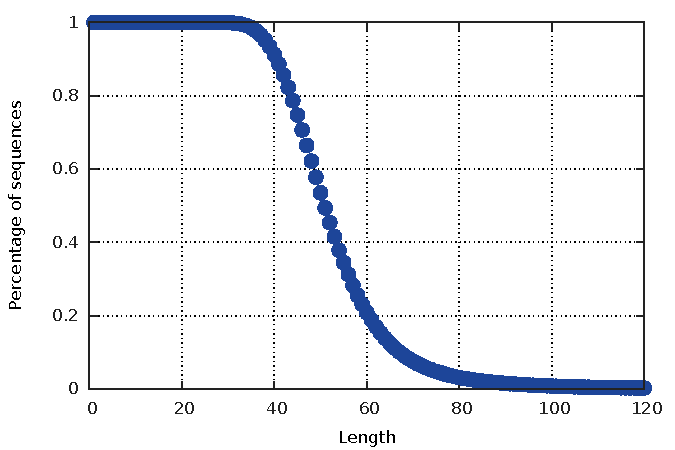
\includegraphics[width=0.7\textwidth]{fig/sequence_length_distribution.pdf}
	\caption{Distribution of caption lengths in the training data.
		\label{fig:length}}
\end{figure}

\section{Pretraining \gls{rnn}} \label{sec:expretrain}

\gls{lstm}-based language model was independently pretrained on captions from the training dataset. Many different versions were trained, varying in count and size of recurrent layers, use of dropout, etc. Most of the variations have similar performance, therefore in this text I will describe only three representative samples. First has two \gls{lstm} layers with 200 units each, second has three layers with 300 units, and third has four layers with 400 units per layer.

All models picked up structure of the text very quickly, generating reasonable English sentences after 50\% of the first epoch. Models were trained for 2 epochs in total, with following captions generated after training:
\vspace{7mm}
\begin{lstlisting}
========SAMPLING=====================================================
A yellow man eating a box, like back of it in the snow.
=====================================================================
========SAMPLING=====================================================
A bathroom with a plate of food in a counter.
=====================================================================
========SAMPLING=====================================================
A couple of men standing on a covered hill with a ramp.
=====================================================================
========SAMPLING=====================================================
A black dog is getting ready to be a graffiti and tree.
=====================================================================
\end{lstlisting}
\vspace{7mm}

\begin{figure}[!t]
	\centering
	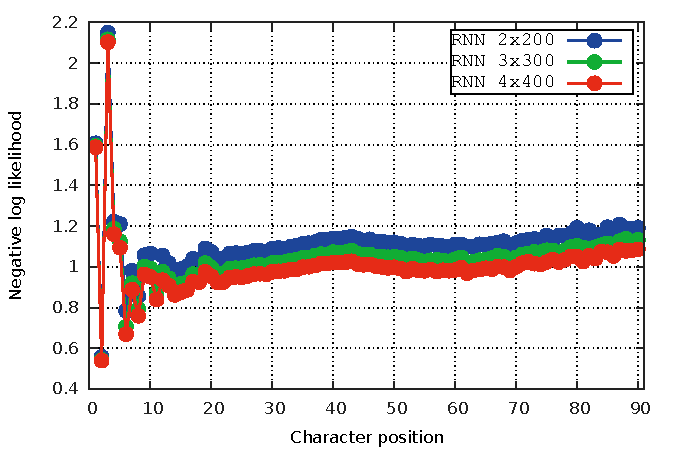
\includegraphics[width=0.7\textwidth]{fig/error_pretraining.pdf}
	\caption{Pretrained \gls{rnn} error based on character position in sequence.
		\label{fig:error_pretrain}}
\end{figure}

Trained models were evaluated on the training dataset by computing average loss for each position of character in the sequence. See the outcomes on Figure \ref{fig:error_pretrain}. Interesting detail on the graph are first three or four positions, which tell that first character of the caption is quite hard to predict, second character is the easiest one and the third most complicated one. This observation can be justified by looking at the training dataset, which has, most of the time, at the beginning the article \textquotedblleft A\textquotedblright\ almost always followed by space \textquotedblleft\ \textquotedblright\ and noun. Space between words is very easy to predict, and on the contrary it is very hard to predict the first character of a word. More general observation is that the error is rising for the first half of the caption and then decline in the second half, as the \gls{rnn} has enough information to predict rest of the sentence.

\subsubsection{Results}

Training multiple character level \gls{rnn} to generate captions, show that smaller networks from two recurrent layers can learn the predictions on the similar level as the larger ones. Larger networks have slight edge in evaluating by negative log likelihood, but have much larger computational cost.

High uncertainty of generation at the beginning of sequence is expected and caused by no prior information about caption being inserted into the network. Generated captions are sometime very unrealistic, but this is again caused by missing knowledge about the real-world. Overall, pretraining \gls{rnn} to random caption generation based on character prediction turned out well, within expected outcomes.

\section{Language model initialization variations} \label{sec:exfullmodel}

\todo[inline]{Udelat}

%th sampling.lua -modelName /storage/brno7-cerit/home/xkvita01/combined_model/0.7244__3x300fc7_1.torch
\vspace{7mm}
\begin{lstlisting}[breakindent=58pt]
========SAMPLING=====================================================
TARGET ++++A railing in front of the beach with surfboards leaning on it.
+++++++++++
SAMPLE ++++there is a suntoking court building is tocmed sestocars lices playing door.
------------------------------------------------------------
TARGET ++++A white and blue train under some palm trees in a city.
+++++++++++
SAMPLE ++++A desk next to a person standing in the field.
------------------------------------------------------------
TARGET ++++A couple of men in a boat going through water, waving at the camera.
+++++++++++
SAMPLE ++++Two clocks and a man base and tracks and small hot dogs.
=====================================================================
\end{lstlisting}
\vspace{7mm}

\subsubsection{Results}
\todo[inline]{Zavery a jak model zlepsit nebo jake experimenty dale provest.}

\section{Bag of Words experiments} \label{sec:exbow}
\todo[inline]{Udelat}

%th sampling.lua -modelName /storage/brno7-cerit/home/xkvita01/combined_model/1.0000__3x300bag1.torch
\vspace{7mm}
\begin{lstlisting}[breakindent=58pt]
========SAMPLING=====================================================
TARGET ++++A person on some skis jumping in the air.
+++++++++++
SAMPLE ++++A person laying at a table with marhorot demilded ebattresss.
------------------------------------------------------------
TARGET ++++A baseball player who just hit the ball running in a baseball game.
+++++++++++
SAMPLE ++++A baseball player in the sliwer ride the board airding a red is parked as their holding the skateboard.
------------------------------------------------------------
TARGET ++++A kitchen with furniture and kitchen accessories and other items.
+++++++++++
SAMPLE ++++A leambed grass forhed  red hicker and a umbrella in a park.
=====================================================================
\end{lstlisting}
\vspace{7mm}

\begin{figure}[!t]
	\centering
	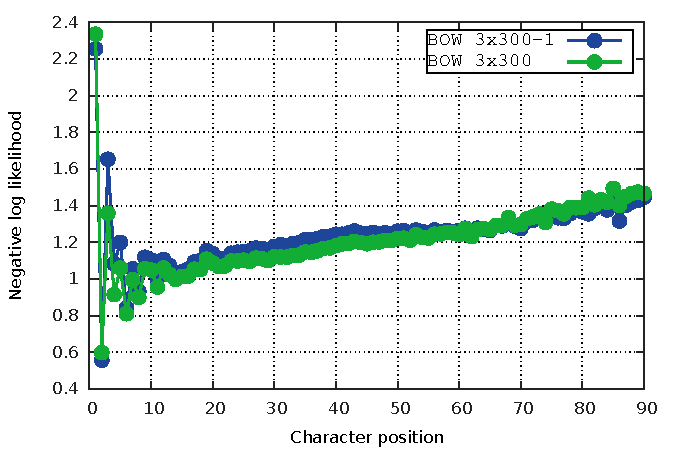
\includegraphics[width=0.7\textwidth]{fig/error_bow.pdf}
	\caption{Error of \gls{rnn} initialized with \gls{bow} based on character position in sequence.
		\label{fig:error_bow}}
\end{figure}

\subsubsection{Results}
\todo[inline]{Udelat}

\chapter{Conclusion}\label{chp:conclusion}

Image captioning is problem more difficult than simple classification of images. Nowadays, deep neural networks are dominating the field almost exclusively. In this work I explained several features of neural networks, which are necessary for creation of image captioning models, and created an overview of the state-of-the-art approaches to this problem. Deep learning is research area with a great need of sufficient datasets, therefore I also listed several biggest and most commonly used. Description part was completed by listing several popular evaluation metrics.

\todo[inline]{Predelat}
\todo[inline]{Ohodnoceni navrhnuteho modelu.}
\todo[inline]{Navrh pro dalsi zmeny ktere by to mohly vylepsit.}


Character level prediction models were created as a building block for creating my own image captioning model, based on the information compiled. I proposed an architecture of the model based on several other approaches, with interest in character level language models instead of word embedding. I explore whether this simple architecture can compete with contemporary solutions focused on word level language models.

In several following months I am planning to work on the details of the convolutional network architecture, implementation and training of the proposed model. Project should be finished by May 2016.


%=========================================================================
